% =========================================================================
% SciPost LaTeX template
% Version 2024-07
%
% Submissions to SciPost Journals should make use of this template.
%
% INSTRUCTIONS: simply look for the `TODO:' tokens and adapt your file.
% ========================================================================

\documentclass{SciPost}

% Prevent all line breaks in inline equations.
\binoppenalty=10000
\relpenalty=10000

\hypersetup{
 colorlinks,
 linkcolor={red!50!black},
 citecolor={blue!50!black},
 urlcolor={blue!80!black}
 }

\usepackage[bitstream-charter]{mathdesign}
\urlstyle{same}

% Fix \cal and \mathcal characters look (so it's not the same as \mathscr)
\DeclareSymbolFont{usualmathcal}{OMS}{cmsy}{m}{n}
\DeclareSymbolFontAlphabet{\mathcal}{usualmathcal}

\fancypagestyle{SPstyle}{
\fancyhf{}
\lhead{\colorbox{scipostblue}{\bf \color{white} ~SciPost Physics }}
\rhead{{\bf \color{scipostdeepblue} ~Submission }}
\renewcommand{\headrulewidth}{1pt}
\fancyfoot[C]{\textbf{\thepage}}
}

\usepackage{graphicx}
\usepackage{tabularx}
\usepackage{subcaption}
\usepackage{placeins}
%DIF 42a42
\usepackage{float} %DIF >
%DIF -------
\usepackage{multirow}
\usepackage{graphbox}
\usepackage{xcolor}
\usepackage{authblk}
\usepackage{tikz-feynman}
\tikzfeynmanset{compat=1.0.0}
\usepackage{hyperref}
%DIF 49d50
%DIF < \usepackage[numbers, sort&compress]{natbib}
%DIF -------

\def\beq{\begin{equation}}
\def\eeq{\end{equation}}
%DIF PREAMBLE EXTENSION ADDED BY LATEXDIFF
%DIF CFONT PREAMBLE %DIF PREAMBLE
\RequirePackage{color}\definecolor{RED}{rgb}{1,0,0}\definecolor{BLUE}{rgb}{0,0,1} %DIF PREAMBLE
\DeclareOldFontCommand{\sf}{\normalfont\sffamily}{\mathsf} %DIF PREAMBLE
\providecommand{\DIFaddtex}[1]{{\protect\color{red} #1}} %DIF PREAMBLE
\providecommand{\DIFdeltex}[1]{} %DIF PREAMBLE
%DIF SAFE PREAMBLE %DIF PREAMBLE
\providecommand{\DIFaddbegin}{} %DIF PREAMBLE
\providecommand{\DIFaddend}{} %DIF PREAMBLE
\providecommand{\DIFdelbegin}{} %DIF PREAMBLE
\providecommand{\DIFdelend}{} %DIF PREAMBLE
\providecommand{\DIFmodbegin}{} %DIF PREAMBLE
\providecommand{\DIFmodend}{} %DIF PREAMBLE
%DIF FLOATSAFE PREAMBLE %DIF PREAMBLE
\providecommand{\DIFaddFL}[1]{\DIFadd{#1}} %DIF PREAMBLE
\providecommand{\DIFdelFL}[1]{\DIFdel{#1}} %DIF PREAMBLE
\providecommand{\DIFaddbeginFL}{} %DIF PREAMBLE
\providecommand{\DIFaddendFL}{} %DIF PREAMBLE
\providecommand{\DIFdelbeginFL}{} %DIF PREAMBLE
\providecommand{\DIFdelendFL}{} %DIF PREAMBLE
%DIF HYPERREF PREAMBLE %DIF PREAMBLE
\providecommand{\DIFadd}[1]{\texorpdfstring{\DIFaddtex{#1}}{#1}} %DIF PREAMBLE
\providecommand{\DIFdel}[1]{\texorpdfstring{\DIFdeltex{#1}}{}} %DIF PREAMBLE
%DIF COLORLISTINGS PREAMBLE %DIF PREAMBLE
\RequirePackage{listings} %DIF PREAMBLE
\RequirePackage{color} %DIF PREAMBLE
\lstdefinelanguage{DIFcode}{ %DIF PREAMBLE
%DIF DIFCODE_CFONT %DIF PREAMBLE
  moredelim=[il][\color{red}\scriptsize]{\%DIF\ <\ }, %DIF PREAMBLE
  moredelim=[il][\color{blue}\sffamily]{\%DIF\ >\ } %DIF PREAMBLE
} %DIF PREAMBLE
\lstdefinestyle{DIFverbatimstyle}{ %DIF PREAMBLE
	language=DIFcode, %DIF PREAMBLE
	basicstyle=\ttfamily, %DIF PREAMBLE
	columns=fullflexible, %DIF PREAMBLE
	keepspaces=true %DIF PREAMBLE
} %DIF PREAMBLE
\lstnewenvironment{DIFverbatim}{\lstset{style=DIFverbatimstyle}}{} %DIF PREAMBLE
\lstnewenvironment{DIFverbatim*}{\lstset{style=DIFverbatimstyle,showspaces=true}}{} %DIF PREAMBLE
%DIF END PREAMBLE EXTENSION ADDED BY LATEXDIFF

\begin{document}

\pagestyle{SPstyle}

\DIFdelbegin %DIFDELCMD < \begin{center}{\Large \textbf{\color{scipostdeepblue}{
%DIFDELCMD < Triple-Higgs production as a probe of the Higgs potential
%DIFDELCMD < }}}%%%
\DIFdelend \DIFaddbegin \begin{center}{\Large \textbf{\color{red}{
Triple-Higgs-boson probes of the Higgs potential and top--Higgs-boson interactions
}}}\DIFaddend \end{center}

\begin{center}\textbf{
{John~M.~Campbell}\textsuperscript{1},
{Giuseppe~De~Laurentis}\textsuperscript{2},
{R.~Keith~Ellis}\textsuperscript{3},
{Michelle Gensmann}\textsuperscript{4,5}\DIFadd{,\ }
{Ulrich~Haisch}\textsuperscript{4$\star$}\DIFadd{,\ }
\DIFadd{{Luca~Panizzi}\textsuperscript{6$\dagger$},\ }
\DIFadd{{Andreas~Papaefstathiou}\textsuperscript{7$\ddagger$} and\ }
\DIFadd{{Gilberto~Tetlalmatzi-Xolocotzi}\textsuperscript{8$\S$}}
}\end{center}

\begin{center}
%%%%%%%%%% TODO: AFFILIATIONS
% Write all affiliations here.
% Format: institute, city, country
{\bf 1 }{Fermilab, PO Box 500, Batavia IL 60510-5011, USA} \\
{\bf 2 }{Higgs Centre for Theoretical Physics, University of Edinburgh, Edinburgh, EH9 3FD, UK} \\
{\bf 3 }{Institute for Particle Physics Phenomenology, Durham University, Durham, DH1 3LE, UK} \\
{\bf 4 }{Max Planck Institute for Physics, Boltzmannstr. 8, 85748 Garching, Germany} \\
{\bf 5 }{Institute for Theoretical Physics, Karlsruhe Institute of Technology, Wolfgang-Gaede-Str. 1, 76131 Karlsruhe, Germany\DIFdelbegin \DIFdel{.}\DIFdelend} \\
\DIFaddbegin \DIFadd{{\bf 6 }{Dipartimento di Fisica, Università della Calabria, I-87036 Arcavacata di Rende, Cosenza, Italy}}\DIFaddend \\
\DIFaddbegin \DIFadd{{\bf 7 }{Department of Physics, Kennesaw State University, 830 Polytechnic Lane, Marietta, GA 30060, USA}}\DIFaddend \\
\DIFaddbegin \DIFadd{{\bf 8 }{Theoretische Physik 1, Center for Particle Physics Siegen (CPPS), Universität Siegen, Walter-Flex-Str.~3, 57068 Siegen, Germany}}\DIFaddend
\\[\baselineskip]
$\star$ \href{mailto:haisch@mpp.mpg.de}{\small haisch@mpp.mpg.de}\DIFaddbegin \DIFadd{\qquad $\dagger$ \href{mailto:luca.panizzi@unical.it}{\textcolor{red}{\small luca.panizzi@unical.it}}}\DIFaddend \\
\DIFaddbegin \DIFadd{$\ddagger$ \href{mailto:apapaefs@kennesaw.edu}{\textcolor{red}{\small apapaefs@kennesaw.edu}} \qquad $\S$ \href{mailto:gtx@physik.uni-siegen.de}{\textcolor{red}{\small gtx@physik.uni-siegen.de}}}\DIFaddend
\end{center}

\begin{center}
 Preprint: FERMILAB-PUB-26-0464-T, LHCHWG-2026-xxx, MPP-2026-xxx
\end{center}

\section*{\color{scipostdeepblue}{Abstract}}
\textbf{\DIFdelbegin %DIFDELCMD < \boldmath{%
%DIFDELCMD < %%%%%%%%%% TODO: ABSTRACT
%DIFDELCMD < % Write your abstract here.
%DIFDELCMD < We study triple-Higgs production in the $\kappa$-framework as a direct probe of the Higgs potential. We derive compact parametrisations of the inclusive gluon-fusion production cross section that capture the dependence on the Higgs trilinear and quartic self-couplings together with anomalous top-Higgs interactions. These results provide a practical framework for interpreting current and future LHC measurements. We use the parametrisations to assess the sensitivity of LHC~Run~2 and HL-LHC data to Higgs self-couplings and show that differential kinematic distributions can provide additional discrimination between scenarios with similar inclusive production rates.
%DIFDELCMD < %%%%%%%%%% END TODO: ABSTRACT
%DIFDELCMD < }%%%
\DIFdelend \DIFaddbegin \boldmath{\color{red}%
%%%%%%%%%% TODO: ABSTRACT
% Write your abstract here.
We study triple-Higgs-boson production in the $\kappa$-framework as a direct probe of the Higgs potential. We derive complementary compact parametrisations of the inclusive gluon-fusion cross section: one retains the dependence on $\kappa_3$, $\kappa_4$, $\kappa_t$, and $\kappa_{2t}$ for $\kappa_{3t}=0$, while the other incorporates $\kappa_{3t}$ for $\kappa_t=1$ and $\kappa_{2t}=0$. These results provide practical tools for interpreting current and future LHC measurements. We use the parametrisations to assess the sensitivity of LHC~Run~2 data and HL-LHC projections to the Higgs boson self-couplings and show that differential kinematic distributions can provide additional discriminatory power between scenarios with nearly identical inclusive production rates.
%%%%%%%%%% END TODO: ABSTRACT
}\DIFaddend }

\vspace{\baselineskip}

%%%%%%%%%% BLOCK: Copyright information
%DIF <  This block will be filled during the proof stage, and finilized just before publication.
%DIF >  This block will be filled during the proof stage, and finalised just before publication.
% It exists here only as a placeholder, and should not be modified by authors.
\noindent\textcolor{white!90!black}{%
\fbox{\parbox{0.975\linewidth}{%
\textcolor{white!40!black}{\begin{tabular}{lr}%
 \begin{minipage}{0.6\textwidth}%
 {\small Copyright attribution to authors. \newline
 This work is a submission to SciPost Physics. \newline
 License information to appear upon publication. \newline
 Publication information to appear upon publication.}
 \end{minipage} & \begin{minipage}{0.4\textwidth}
 {\small Received Date \newline Accepted Date \newline Published Date}%
 \end{minipage}
\end{tabular}}
}}
}
%%%%%%%%%% BLOCK: Copyright information


%%%%%%%%%% TODO: LINENO
% For convenience during refereeing we turn on line numbers:
%\linenumbers
% You should run LaTeX twice in order for the line numbers to appear.
%%%%%%%%%% END TODO: LINENO

%%%%%%%%%% TODO: TOC
%DIF <  Guideline: if your paper is longer that 6 pages, include a TOC
%DIF >  Guideline: if your paper is longer than 6 pages, include a TOC
% To remove the TOC, simply cut the following block

\newpage

\vspace{10pt}
\noindent\rule{\textwidth}{1pt}
\tableofcontents
\noindent\rule{\textwidth}{1pt}
\vspace{10pt}
%%%%%%%%%% END TODO: TOC

\allowdisplaybreaks

\section{\textbf{\boldmath{Introduction}}}
\label{sec:introduction}

The discovery of the Higgs boson in 2012~\cite{ATLAS:2012yve,CMS:2012qbp} completed the particle content of the Standard Model~(SM) and established the mechanism of electroweak~(EW) symmetry breaking. Since~then, a major objective of the LHC physics programme has been to determine the properties of the Higgs boson with increasing precision. While its couplings to EW gauge bosons and third-generation fermions are already constrained at the few- to ten-percent level, its self-interactions remain largely unexplored. Measuring the Higgs \DIFaddbegin \DIFadd{boson }\DIFaddend self-couplings is therefore one of the most important outstanding goals of collider physics, since they directly probe the shape of the Higgs potential and the dynamics of EW symmetry breaking.

In the SM, the Higgs potential is determined by a single quartic coupling $\lambda = m_h^2/(2v^2)$. After EW symmetry breaking, it predicts unique values for the Higgs \DIFaddbegin \DIFadd{boson }\DIFaddend trilinear and quartic self-couplings,
\beq \label{eq:SM67}
\lambda_3^{\DIFdelbegin %DIFDELCMD < \rm %%%
\DIFdel{SM}\DIFdelend \DIFaddbegin \DIFadd{\mathrm{SM}}\DIFaddend } = \lambda \,, \qquad
\lambda_4^{\DIFdelbegin %DIFDELCMD < \rm %%%
\DIFdel{SM}\DIFdelend \DIFaddbegin \DIFadd{\mathrm{SM}}\DIFaddend } = \frac{\lambda}{4} \,,
\eeq
once the Higgs boson mass $m_h\simeq125\,\mathrm{GeV}$ and vacuum expectation value $v\simeq246\,\mathrm{GeV}$ are fixed. Any deviation from these predictions would provide evidence for physics beyond the SM, such as extended scalar sectors, composite Higgs models, or mechanisms for EW baryogenesis. Reviews of such beyond-the-SM~(BSM) scenarios can be found, for example, in~Refs.~\cite{DiMicco:2019ngk,Durieux:2022hbu}.

At the LHC, \DIFdelbegin \DIFdel{double-Higgs }\DIFdelend \DIFaddbegin \DIFadd{double-Higgs-boson }\DIFaddend production provides the primary direct probe of the Higgs \DIFaddbegin \DIFadd{boson }\DIFaddend trilinear self-coupling, while loop-induced effects in \DIFdelbegin \DIFdel{single-Higgs }\DIFdelend \DIFaddbegin \DIFadd{single-Higgs-boson }\DIFaddend processes yield complementary constraints~\cite{Gorbahn:2016uoy,Degrassi:2016wml,Bizon:2016wgr,Maltoni:2017ims,Gorbahn:2019lwq,Haisch:2021hvy,Gao:2023bll,Haisch:2024nzv,Ghosh:2025fma}. These measurements are typically interpreted in the $\kappa$-framework~\cite{LHCHiggsCrossSectionWorkingGroup:2012nn,LHCHiggsCrossSectionWorkingGroup:2013rie,LHCHiggsCrossSectionWorkingGroup:2016ypw}, which parametrises deviations from the SM through
\beq \label{eq:kappa3}
\kappa_3 = \DIFdelbegin \DIFdel{\frac{\lambda_3}{\lambda_3^{\rm SM}} }\DIFdelend \DIFaddbegin \DIFadd{\frac{\lambda_3}{\lambda_3^{\mathrm{SM}}} }\DIFaddend \,,
\eeq
assuming all other couplings take their SM values. Using the full $\sqrt{s}=13\,\mathrm{TeV}$ LHC~Run~2 data set, the ATLAS and CMS collaborations obtain the combined constraint
\beq \label{eq:kappa3bound}
-0.71 < \kappa_3 < 6.1\;\;\;(\text{ATLAS}+\text{CMS})
\eeq
at \DIFdelbegin \DIFdel{the }\DIFdelend $95\%$ confidence level~(CL)~\cite{CMS:2026nuu}. The HL-LHC, with an integrated luminosity of \DIFaddbegin \DIFadd{$3\,\mathrm{ab}^{-1}$ per experiment, corresponding to a combined ATLAS--CMS exposure of }\DIFaddend $6\,\mathrm{ab}^{-1}$, is expected to improve this sensitivity to
\beq
0.5 < \kappa_3 < 1.7\;\;\;(\text{HL-LHC})\,.
\eeq
\DIFaddbegin \DIFadd{This projection is taken from~Ref.~\cite{ATL-PHYS-PUB-2025-018}.
}\DIFaddend

Constraining the quartic Higgs \DIFaddbegin \DIFadd{boson }\DIFaddend self-coupling is considerably more challenging. It is conventionally parametrised as
\beq \label{eq:kappa4}
\kappa_4 = \DIFdelbegin \DIFdel{\frac{\lambda_4}{\lambda_4^{\rm SM}} }\DIFdelend \DIFaddbegin \DIFadd{\frac{\lambda_4}{\lambda_4^{\mathrm{SM}}} }\DIFaddend \,,
\eeq
and \DIFdelbegin \DIFdel{triple-Higgs }\DIFdelend \DIFaddbegin \DIFadd{triple-Higgs-boson }\DIFaddend production provides its only direct probe at hadron colliders. However, the tiny SM cross section of approximately $100\,\mathrm{ab}$ at $\sqrt{s}=14\,\mathrm{TeV}$, calculated at next-to-next-to-leading order~(NNLO) in QCD~\cite{deFlorian:2019app}, renders such measurements experimentally very challenging. Current ATLAS~\cite{ATLAS:2024xcs} and CMS~\cite{CMS-PAS-HIG-24-012} searches yield
\beq \label{eq:kappa4bounds}
-230 < \kappa_4 < 240 \;\;\;(\DIFdelbegin %DIFDELCMD < \rm %%%
\DIFdel{ATLAS}\DIFdelend \DIFaddbegin \DIFadd{\text{ATLAS}}\DIFaddend ) \,, \qquad
-190 < \kappa_4 < 190 \;\;\;(\DIFdelbegin %DIFDELCMD < \rm %%%
\DIFdel{CMS}\DIFdelend \DIFaddbegin \DIFadd{\text{CMS}}\DIFaddend ) \,,
\eeq
at \DIFdelbegin \DIFdel{the }\DIFdelend $95\%$~CL, assuming all other couplings are SM-like, in particular $\kappa_3=1$. A recent HL-LHC study~\cite{Ding:2026qto} projects these bounds to improve to
\beq \DIFaddbegin \label{eq:kappa4boundsHL}
\DIFaddend -81 < \kappa_4 < 89\;\;\;(\text{HL-LHC})
\eeq
\DIFdelbegin \DIFdel{with an integrated luminosity }\DIFdelend \DIFaddbegin \DIFadd{for a combined ATLAS--CMS exposure }\DIFaddend of $6\,\mathrm{ab}^{-1}$\DIFaddbegin \DIFadd{, corresponding to $3\,\mathrm{ab}^{-1}$ per experiment}\DIFaddend . In addition to \DIFdelbegin \DIFdel{triple-Higgs production, double-Higgs }\DIFdelend \DIFaddbegin \DIFadd{triple-Higgs-boson production, double-Higgs-boson }\DIFaddend production is also sensitive to $\kappa_4$ through two-loop EW corrections~\cite{Bizon:2018syu,Borowka:2018pxx,Li:2024iio,Ding:2026qto}, although these constraints are generally weaker.

In this note, we present a comprehensive study of \DIFdelbegin \DIFdel{triple-Higgs }\DIFdelend \DIFaddbegin \DIFadd{triple-Higgs-boson }\DIFaddend production within the $\kappa$-framework. We derive \DIFaddbegin \DIFadd{complementary }\DIFaddend compact parametrisations of the inclusive gluon-fusion \DIFdelbegin \DIFdel{production cross sectionthat capture its }\DIFdelend \DIFaddbegin \DIFadd{cross section. The first retains the }\DIFaddend dependence on the Higgs \DIFaddbegin \DIFadd{boson }\DIFaddend trilinear and quartic self-couplings, the top-quark Yukawa coupling modifier $\kappa_t$, and the \DIFdelbegin \DIFdel{two-top-two-Higgs }\DIFdelend \DIFaddbegin \DIFadd{two-top--two-Higgs-boson }\DIFaddend interaction $\kappa_{2t}$ \DIFaddbegin \DIFadd{for $\kappa_{3t}=0$. The second incorporates the two-top--three-Higgs-boson interaction $\kappa_{3t}$ for $\kappa_t=1$ and $\kappa_{2t}=0$}\DIFaddend . These~expressions provide practical tools for interpreting current and future LHC measurements. Using them, we investigate the sensitivity of current \DIFdelbegin \DIFdel{and projected LHC data}\DIFdelend \DIFaddbegin \DIFadd{LHC data and HL-LHC projections}\DIFaddend  to the Higgs \DIFaddbegin \DIFadd{boson }\DIFaddend self-couplings and study the impact of correlated modifications of \DIFdelbegin \DIFdel{$\kappa_t$ and $\kappa_{2t}$}\DIFdelend \DIFaddbegin \DIFadd{the top--Higgs-boson interactions}\DIFaddend . We further demonstrate that differential kinematic distributions retain significant sensitivity \DIFdelbegin \DIFdel{to the Higgs potential }\DIFdelend even in scenarios with nearly degenerate inclusive cross sections, highlighting the importance of shape information in future \DIFdelbegin \DIFdel{triple-Higgs }\DIFdelend \DIFaddbegin \DIFadd{triple-Higgs-boson }\DIFaddend searches.

\section{\DIFdelbegin \DIFdel{\textbf{\boldmath{Triple-Higgs production in the $\kappa$-framework}}}\DIFdelend \DIFaddbegin \texorpdfstring{\textbf{\boldmath{Triple-Higgs-boson production in the $\kappa$-framework}}}{Triple-Higgs-boson production in the kappa-framework}\DIFaddend }
\label{sec:results}

\begin{figure}[t!]
\begin{center}
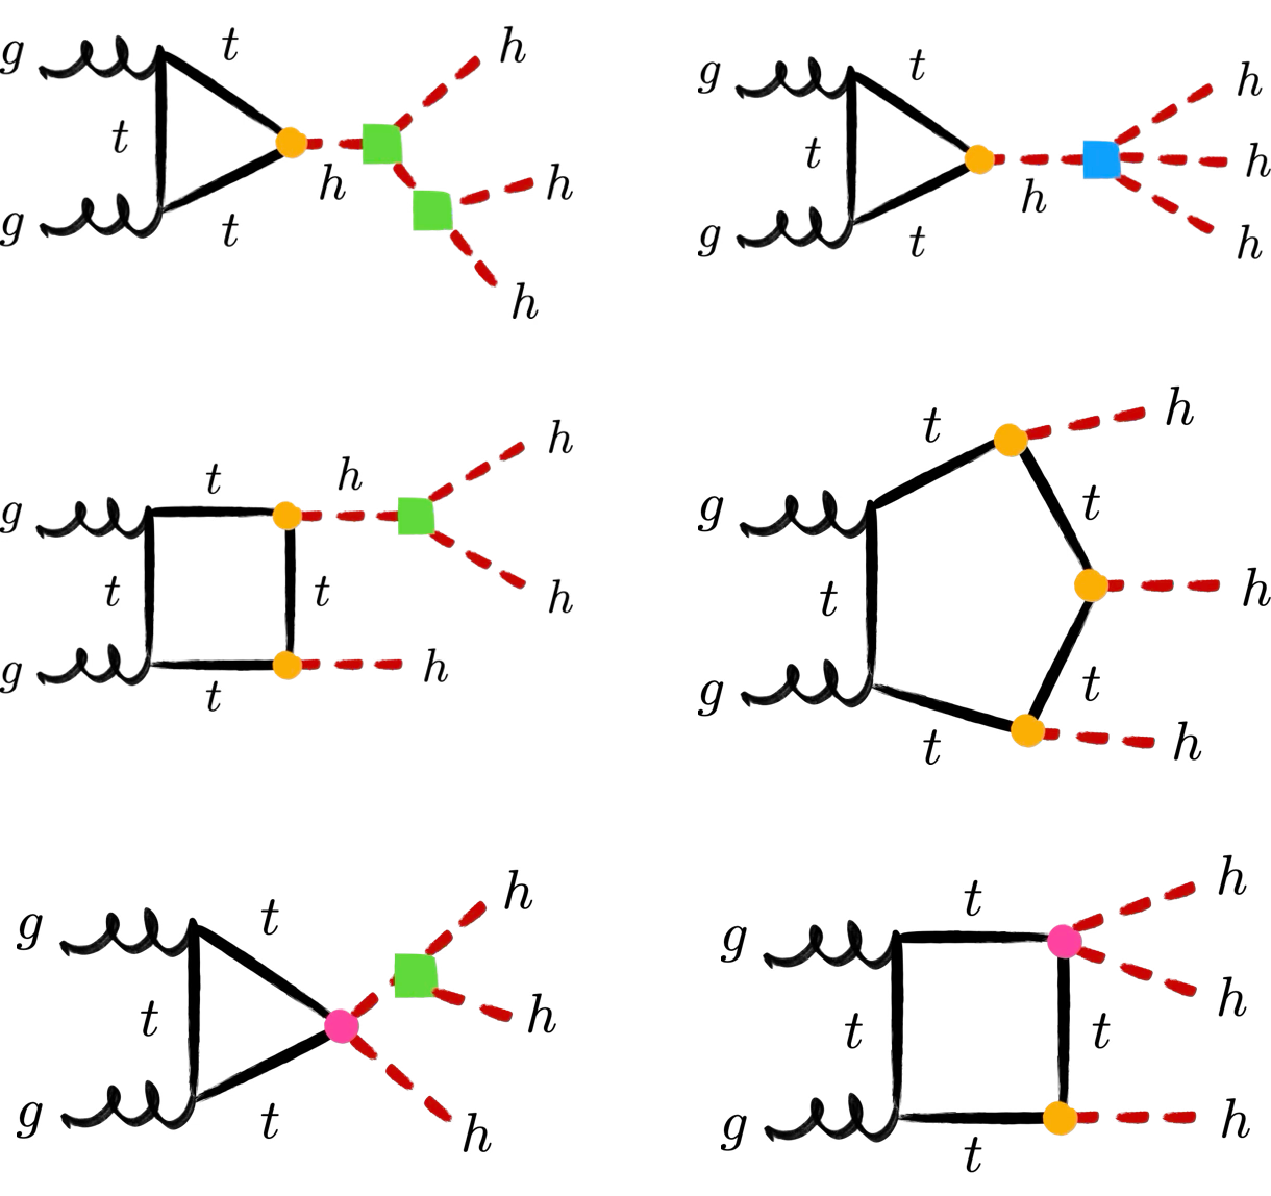
\includegraphics[width=0.85\textwidth]{diagrams.pdf}
\end{center}
\vspace{2mm}
\caption{\label{fig:diagrams} Representative one-loop Feynman diagrams contributing to \DIFdelbeginFL \DIFdelFL{triple-Higgs }\DIFdelendFL \DIFaddbeginFL \DIFaddFL{triple-Higgs-boson }\DIFaddendFL production via gluon fusion, illustrating the triangle, box, and pentagon topologies. Green (blue) boxes denote the Higgs \DIFaddbeginFL \DIFaddFL{boson }\DIFaddendFL trilinear (quartic) self-coupling, while orange (magenta) circles indicate top-quark couplings involving one (two) Higgs bosons.}
\end{figure}

\DIFdelbegin \DIFdel{Triple-Higgs }\DIFdelend \DIFaddbegin \DIFadd{Triple-Higgs-boson }\DIFaddend production at hadron colliders has been the subject of extensive theoretical investigation over the past two decades~\cite{Plehn:2005nk,Binoth:2006ym,Maltoni:2014eza,Papaefstathiou:2015paa,Chen:2015gva,Fuks:2015hna,deFlorian:2016sit,Kilian:2017nio,Fuks:2017zkg,Bizon:2018syu,deFlorian:2019app,Stylianou:2023xit,Papaefstathiou:2023uum,Abouabid:2024gms,Dong:2025lkm,Haisch:2025pql,Campbell:2025llb,Fuks:2025gjv,Panizzi:2025sya,Ding:2026qto}. Within the SM, the gluon-fusion process $gg \to 3h$ is dominated by the one-loop topologies shown in the upper and middle rows of Figure~\ref{fig:diagrams}. In the figure, green (blue) boxes denote insertions of the Higgs \DIFaddbegin \DIFadd{boson }\DIFaddend trilinear (quartic) self-coupling, while orange circles represent the top-quark Yukawa coupling. The two diagrams in the lower row illustrate representative BSM contributions involving a contact interaction between two top quarks and two Higgs bosons. In the SM, bottom-quark loops \DIFdelbegin \DIFdel{contribute only about $-0.2\%$ to }\DIFdelend \DIFaddbegin \DIFadd{modify }\DIFaddend the $gg \to 3h$ production cross section \DIFaddbegin \DIFadd{by only about $0.2\%$ }\DIFaddend at LHC energies~\cite{Campbell:2025llb}\DIFdelbegin \DIFdel{. We therefore neglect all light-quark contributions throughout the remainder of this work}\DIFdelend \DIFaddbegin \DIFadd{; they are nevertheless retained in the numerical calculations below}\DIFaddend .

The \DIFaddbegin \DIFadd{relevant terms in the }\DIFaddend $\kappa$\DIFdelbegin \DIFdel{-formalism Lagrangian, which parametrises the interaction vertices highlighted in ~Figure~\ref{fig:diagrams}, takes the form
}\DIFdelend \DIFaddbegin \DIFadd{-framework Lagrangian are
}\DIFaddend \beq \label{eq:Lkappa}
{\cal L}_{\kappa} \supset -\kappa_3 \hspace{0.25mm} v \lambda h^3 -\kappa_4 \hspace{0.25mm} \frac{\lambda}{4} \hspace{0.5mm} h^4 -\kappa_t \hspace{0.25mm} \frac{y_t}{\sqrt{2}} \hspace{0.5mm} \bar t t h  -\kappa_{2t} \hspace{0.25mm} \frac{y_t}{\sqrt{2} \hspace{0.25mm} v} \hspace{0.5mm} \bar t t h^2 \DIFaddbegin \DIFadd{-\kappa_{3t} \hspace{0.25mm} \frac{y_t}{2\sqrt{2} \hspace{0.25mm} v^2} \hspace{0.5mm} \bar t t h^3 }\DIFaddend \,,
\eeq
where $\kappa_3$ and $\kappa_4$ were introduced in~Eqs.~(\ref{eq:kappa3}) and (\ref{eq:kappa4}), respectively, and $y_t = \sqrt{2} \hspace{0.125mm} m_t/v$, with $m_t$ denoting the top-quark mass. The parameter $\kappa_t$ thus encodes modifications of the top-quark Yukawa coupling, while \DIFdelbegin \DIFdel{the parameter }\DIFdelend $\kappa_{2t}$ \DIFdelbegin \DIFdel{parametrises the coupling }\DIFdelend \DIFaddbegin \DIFadd{and $\kappa_{3t}$ parametrise contact interactions }\DIFaddend between two top quarks and two \DIFdelbegin \DIFdel{Higgs bosons}\DIFdelend \DIFaddbegin \DIFadd{or three Higgs bosons, respectively. The final term can equivalently be written as $-\kappa_{3t}m_t\bar t t h^3/(2v^3)$~\cite{Papaefstathiou:2023uum}}\DIFaddend . The SM is recovered from~Eq.~(\ref{eq:Lkappa}) for $\kappa_3 = \kappa_4 = \kappa_t = 1$ and \DIFdelbegin \DIFdel{$\kappa_{2t} = 0$}\DIFdelend \DIFaddbegin \DIFadd{$\kappa_{2t} = \kappa_{3t} = 0$}\DIFaddend .

\begin{figure}[t!]
\begin{center}
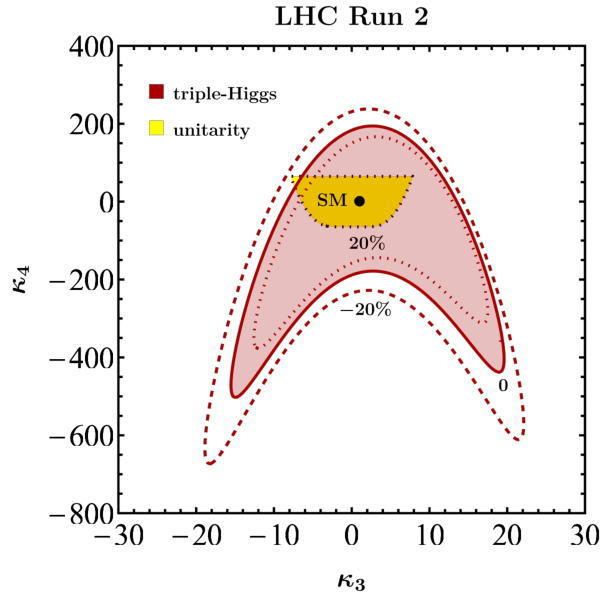
\includegraphics[width=0.45\textwidth]{LHCRun2_3h_YR5.pdf} \quad
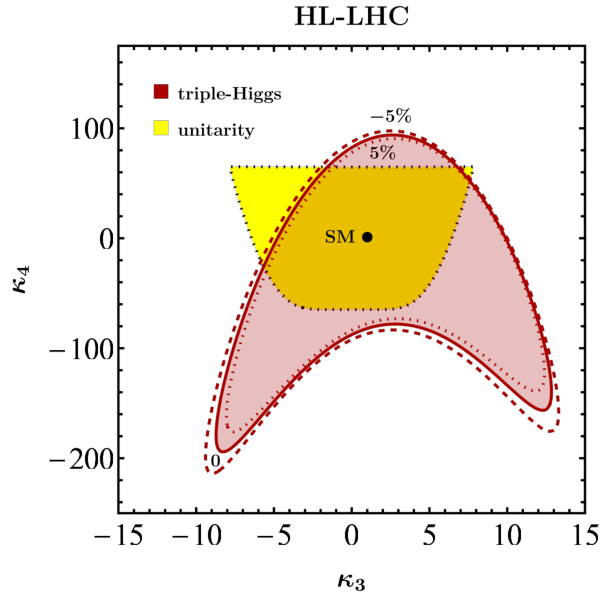
\includegraphics[width=0.45\textwidth]{HLLHC_3h_YR5.pdf}
\end{center}
\vspace{-4mm}
\caption{\label{fig:planes} Constraints in the $\kappa_3\hspace{0.25mm}$--$\hspace{0.25mm}\kappa_4$ plane at LHC~Run~2~(left) and the HL-LHC~(right). The red contours indicate the \DIFdelbeginFL \DIFdelFL{preferred }\DIFdelendFL \DIFaddbeginFL \DIFaddFL{allowed }\DIFaddendFL $95\%$\DIFaddbeginFL \DIFaddFL{~}\DIFaddendFL CL regions obtained from \DIFdelbeginFL \DIFdelFL{triple-Higgs }\DIFdelendFL \DIFaddbeginFL \DIFaddFL{triple-Higgs-boson }\DIFaddendFL production in gluon fusion for three representative values of $\kappa_t$, as specified by the contour labels. We assume \DIFdelbeginFL \DIFdelFL{$\kappa_{2t}=0$}\DIFdelendFL \DIFaddbeginFL \DIFaddFL{$\kappa_{2t}=\kappa_{3t}=0$}\DIFaddendFL . The SM prediction is denoted by black points. The yellow regions, enclosed by black dotted contours, represent the \DIFdelbeginFL \DIFdelFL{perturbative unitarity }\DIFdelendFL \DIFaddbeginFL \DIFaddFL{perturbative-unitarity }\DIFaddendFL bounds derived from tree-level $hh\to hh$ scattering.}
\end{figure}

To determine the dependence of the inclusive $gg \to 3h$ production cross section on $\kappa_3$, $\kappa_4$, $\kappa_t$, and $\kappa_{2t}$, we employ the leading-order~(LO) matrix elements calculated in~Ref.~\cite{Campbell:2025llb} and implemented in the \DIFdelbegin %DIFDELCMD < {\tt %%%
\DIFdel{MCFM}%DIFDELCMD < }%%%
\DIFdelend \DIFaddbegin \DIFadd{\texttt{MCFM}}\DIFaddend ~\cite{Campbell:1999ah,Campbell:2011bn,Campbell:2015qma,Campbell:2019dru} parton-level event generator. We use $m_h = 125\,\mathrm{GeV}$ and $m_t = 173\,\mathrm{GeV}$ as input parameters together with the \DIFdelbegin %DIFDELCMD < {\tt %%%
\DIFdel{PDF4LHC21}%DIFDELCMD < } %%%
\DIFdelend \DIFaddbegin \DIFadd{\texttt{PDF4LHC21} }\DIFaddend parton distribution functions~(PDFs)~\cite{PDF4LHCWorkingGroup:2022cjn}. The renormalisation and factorisation scales, $\mu_R$ and $\mu_F$, are chosen dynamically as $\mu_R = \mu_F = m_{3h}/2$, where $m_{3h}$ denotes the invariant mass of the \DIFdelbegin \DIFdel{three-Higgs system. For collision energies of }\DIFdelend \DIFaddbegin \DIFadd{three-Higgs-boson system. At centre-of-mass energies }\DIFaddend $\sqrt{s}=13\,\mathrm{TeV}$, \DIFdelbegin \DIFdel{$\sqrt{s}=13.6\,\mathrm{TeV}$, and $\sqrt{s}=14\,\mathrm{TeV}$}\DIFdelend \DIFaddbegin \DIFadd{$13.6\,\mathrm{TeV}$, and $14\,\mathrm{TeV}$, and with $\kappa_{3t}=0$}\DIFaddend , we parametrise the LO cross section as
\beq \label{eq:BSMLO}
\sigma_{\mathrm{LO}}^{\sqrt{s}} = \big(\sigma_{\mathrm{LO}}^{\sqrt{s}}\big)_{\DIFdelbegin %DIFDELCMD < \rm %%%
\DIFdel{SM}\DIFdelend \DIFaddbegin \DIFadd{\mathrm{SM}}\DIFaddend } \sum_{n,m} c_{nm}^{\sqrt{s}}\!\left(\kappa_t,\kappa_{2t}\right) \big(\Delta\kappa_3\big)^n \big(\Delta\kappa_4\big)^m \,,
\eeq
where $\Delta\kappa_i=\kappa_i-1$ for $i=3,4$. The corresponding LO SM cross sections are
\beq \label{eq:SMLO}
\sigma_{\mathrm{LO}}^{13\,\mathrm{TeV}} = 42.1\,\mathrm{ab} \,, \qquad
\sigma_{\mathrm{LO}}^{13.6\,\mathrm{TeV}} = 47.9\,\mathrm{ab} \,, \qquad
\sigma_{\mathrm{LO}}^{14\,\mathrm{TeV}} = 51.0\,\mathrm{ab} \,.
\eeq

For $\sqrt{s} = 13\,\mathrm{TeV}$, the coefficients $c_{nm}^{\sqrt{s}}\big(\kappa_t,\kappa_{2t}\big)$ appearing in~Eq.~(\ref{eq:BSMLO}) are
\begin{align}
c_{00}^{13\,\mathrm{TeV}} \big(\kappa_t,\kappa_{2t}\big) & =
-6.05\times10^{-4}
+0.0384\hspace{0.25mm}\kappa_t^2
-0.350\hspace{0.25mm}\kappa_t^3
+1.47\hspace{0.25mm}\kappa_t^4
-3.04\hspace{0.25mm}\kappa_t^5
+2.89\hspace{0.25mm}\kappa_t^6 \notag \\[1mm]
& \phantom{=} +\kappa_{2t}
\left(
1.61\hspace{0.25mm}\kappa_t^2
-7.82\hspace{0.25mm}\kappa_t^3
+15.6\hspace{0.25mm}\kappa_t^4
-14.8\hspace{0.25mm}\kappa_t^5
\right) \notag \\[1mm]
& \phantom{=} +\kappa_{2t}^2
\left(
6.96
-22.3\hspace{0.25mm}\kappa_t
+37.0\hspace{0.25mm}\kappa_t^2
\right) \,, \label{eq:c00_13} \\[2mm]
c_{01}^{13\,\mathrm{TeV}} \big(\kappa_t,\kappa_{2t}\big) & =
0.0829\hspace{0.25mm}\kappa_t^2
-0.264\hspace{0.25mm}\kappa_t^3
+0.0895\hspace{0.25mm}\kappa_t^4
+\kappa_{2t}
\left(
0.673\hspace{0.25mm}\kappa_t
-1.12\hspace{0.25mm}\kappa_t^2
\right) \,, \label{eq:c01_13} \\[2mm]
c_{02}^{13\,\mathrm{TeV}} \big(\kappa_t,\kappa_{2t}\big) & =
0.0169\hspace{0.25mm}\kappa_t^2 \,, \label{eq:c02_13} \\[2mm]
c_{10}^{13\,\mathrm{TeV}} \big(\kappa_t,\kappa_{2t}\big) & =
0.211\hspace{0.25mm}\kappa_t^2
-1.45\hspace{0.25mm}\kappa_t^3
+3.65\hspace{0.25mm}\kappa_t^4
-3.28\hspace{0.25mm}\kappa_t^5 \notag \\[1mm]
& \phantom{=} +\kappa_{2t}
\left(
3.49\hspace{0.25mm}\kappa_t
-13.4\hspace{0.25mm}\kappa_t^2
+15.6\hspace{0.25mm}\kappa_t^3
\right) +
\kappa_{2t}^2
\left(
13.9
-22.3\hspace{0.25mm}\kappa_t
\right) \,, \label{eq:c10_13} \\[2mm]
c_{11}^{13\,\mathrm{TeV}} \big(\kappa_t,\kappa_{2t}\big) & =
0.0978\hspace{0.25mm}\kappa_t^2
-0.264\hspace{0.25mm}\kappa_t^3
+ 0.673\hspace{0.25mm}\kappa_{2t}\hspace{0.125mm}\kappa_t \,, \label{eq:c11_13} \\[2mm]
c_{20}^{13\,\mathrm{TeV}} \big(\kappa_t,\kappa_{2t}\big) & =
0.288\hspace{0.25mm}\kappa_t^2
-1.25\hspace{0.25mm}\kappa_t^3
+1.84\hspace{0.25mm}\kappa_t^4
+\kappa_{2t}
\left(
2.81\hspace{0.25mm}\kappa_t
-6.70\hspace{0.25mm}\kappa_t^2
\right)
+6.96\hspace{0.25mm}\kappa_{2t}^2 \,, \label{eq:c20_13} \\[2mm]
c_{21}^{13\,\mathrm{TeV}} \big(\kappa_t,\kappa_{2t}\big) & =
0.0489\hspace{0.25mm}\kappa_t^2 \,, \label{eq:c21_13} \\[2mm]
c_{30}^{13\,\mathrm{TeV}} \big(\kappa_t,\kappa_{2t}\big) & =
0.159\hspace{0.25mm}\kappa_t^2
-0.417\hspace{0.25mm}\kappa_t^3
+0.938\hspace{0.25mm}\kappa_{2t}\hspace{0.125mm}\kappa_t \,, \label{eq:c30_13} \\[2mm]
c_{40}^{13\,\mathrm{TeV}} \big(\kappa_t,\kappa_{2t}\big) & =
0.0396\hspace{0.25mm} \kappa_t^2 \label{eq:c40_13} \,.
\end{align}

\begin{figure}[t!]
\begin{center}
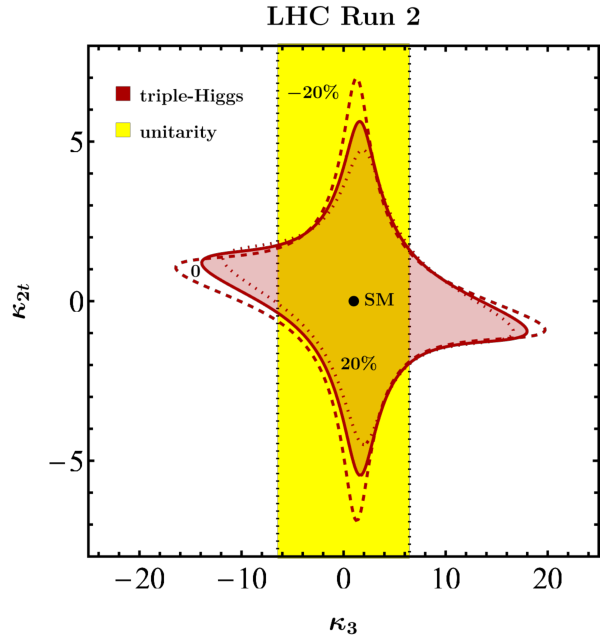
\includegraphics[width=0.45\textwidth]{LHCRun2_k3k2t_3h_YR5.pdf} \quad
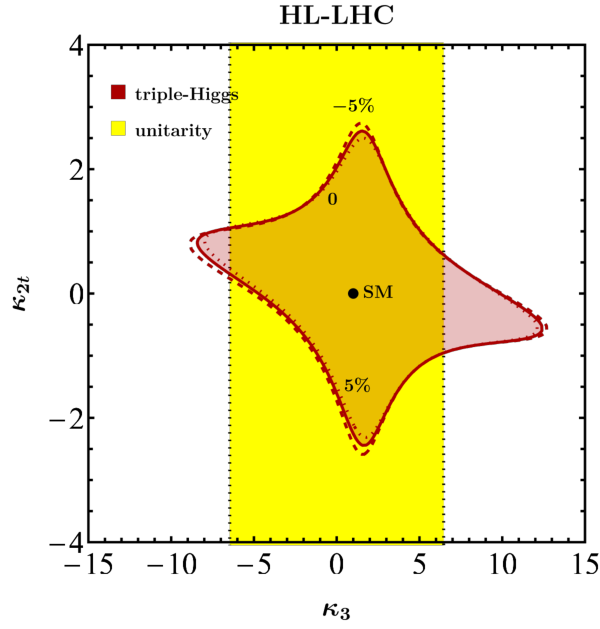
\includegraphics[width=0.45\textwidth]{HLLHC_k3k2t_3h_YR5.pdf}
\end{center}
\vspace{-4mm}
\caption{\label{fig:planes2} As \DIFaddbeginFL \DIFaddFL{in~}\DIFaddendFL Figure~\ref{fig:planes}, but in the $\kappa_3\hspace{0.25mm}$--$\hspace{0.25mm}\kappa_{2t}$ plane at LHC~Run~2~(left) and the HL-LHC~(right). The parameters not shown explicitly are fixed to their SM values, i.e.~\DIFdelbeginFL \DIFdelFL{$\kappa_4=1$ }\DIFdelendFL \DIFaddbeginFL \DIFaddFL{$\kappa_4=\kappa_t=1$ }\DIFaddendFL and \DIFdelbeginFL \DIFdelFL{$\kappa_t=1$}\DIFdelendFL \DIFaddbeginFL \DIFaddFL{$\kappa_{3t}=0$}\DIFaddendFL .}
\end{figure}

At $\sqrt{s} = 13.6\,\mathrm{TeV}$, the corresponding coefficients read
\begin{align}
c_{00}^{13.6\,\mathrm{TeV}} \big(\kappa_t,\kappa_{2t}\big) & =
-9.34\times10^{-3}
+0.0572\hspace{0.25mm}\kappa_t^2
-0.446\hspace{0.25mm}\kappa_t^3
+1.68\hspace{0.25mm}\kappa_t^4
-3.17\hspace{0.25mm}\kappa_t^5
+2.89\hspace{0.25mm}\kappa_t^6 \notag \\[1mm]
& \phantom{=} +\kappa_{2t}
\left(
1.59\hspace{0.25mm}\kappa_t^2
-7.69\hspace{0.25mm}\kappa_t^3
+15.3\hspace{0.25mm}\kappa_t^4
-14.6\hspace{0.25mm}\kappa_t^5
\right) \notag \\[1mm]
& \phantom{=} +\kappa_{2t}^2
\left(
6.89
-22.1\hspace{0.25mm}\kappa_t
+36.8\hspace{0.25mm}\kappa_t^2
\right) \,, \label{eq:c00_136} \\[2mm]
c_{01}^{13.6\,\mathrm{TeV}} \big(\kappa_t,\kappa_{2t}\big) & =
0.0814\hspace{0.25mm}\kappa_t^2
-0.260\hspace{0.25mm}\kappa_t^3
+0.0866\hspace{0.25mm}\kappa_t^4
+\kappa_{2t}
\left(
0.665\hspace{0.25mm}\kappa_t
-1.10\hspace{0.25mm}\kappa_t^2
\right) \,, \label{eq:c01_136} \\[2mm]
c_{02}^{13.6\,\mathrm{TeV}} \big(\kappa_t,\kappa_{2t}\big) & =
0.0167\hspace{0.25mm}\kappa_t^2 \,, \label{eq:c02_136} \\[2mm]
c_{10}^{13.6\,\mathrm{TeV}} \big(\kappa_t,\kappa_{2t}\big) & =
0.204\hspace{0.25mm}\kappa_t^2
-1.40\hspace{0.25mm}\kappa_t^3
+3.56\hspace{0.25mm}\kappa_t^4
-3.21\hspace{0.25mm}\kappa_t^5 \notag \\[1mm]
& \phantom{=} +\kappa_{2t}
\left(
3.43\hspace{0.25mm}\kappa_t
-13.2\hspace{0.25mm}\kappa_t^2
+15.3\hspace{0.25mm}\kappa_t^3
\right)
+\kappa_{2t}^2
\left(
13.8
-22.1\hspace{0.25mm}\kappa_t
\right) \,, \label{eq:c10_136} \\[2mm]
c_{11}^{13.6\,\mathrm{TeV}} \big(\kappa_t,\kappa_{2t}\big) & =
0.0961\hspace{0.25mm}\kappa_t^2
-0.260\hspace{0.25mm}\kappa_t^3
+ 0.665\hspace{0.25mm}\kappa_{2t}\hspace{0.125mm}\kappa_t \,, \label{eq:c11_136} \\[2mm]
c_{20}^{13.6\,\mathrm{TeV}} \big(\kappa_t,\kappa_{2t}\big) & =
0.283\hspace{0.25mm}\kappa_t^2
-1.23\hspace{0.25mm}\kappa_t^3
+1.81\hspace{0.25mm}\kappa_t^4
+\kappa_{2t}
\left(
2.77\hspace{0.25mm}\kappa_t
-6.59\hspace{0.25mm}\kappa_t^2
\right)
+6.89\hspace{0.25mm}\kappa_{2t}^2 \,, \label{eq:c20_136} \\[2mm]
c_{21}^{13.6\,\mathrm{TeV}} \big(\kappa_t,\kappa_{2t}\big) & =
0.0480\hspace{0.25mm}\kappa_t^2 \,, \label{eq:c21_136} \\[2mm]
c_{30}^{13.6\,\mathrm{TeV}} \big(\kappa_t,\kappa_{2t}\big) & =
0.155\hspace{0.25mm}\kappa_t^2
-0.408\hspace{0.25mm}\kappa_t^3
+0.922\hspace{0.25mm}\kappa_{2t}\hspace{0.125mm}\kappa_t \,, \label{eq:c30_136} \\[2mm]
c_{40}^{13.6\,\mathrm{TeV}} \big(\kappa_t,\kappa_{2t}\big) & =
0.0388\hspace{0.25mm} \kappa_t^2 \label{eq:c40_136} \,.
\end{align}

Finally, for $\sqrt{s} = 14\,\mathrm{TeV}$, we obtain
\begin{align}
c_{00}^{14\,\mathrm{TeV}} \big(\kappa_t,\kappa_{2t}\big) & =
-2.18\times10^{-3}
+0.0323\hspace{0.25mm}\kappa_t^2
-0.311\hspace{0.25mm}\kappa_t^3
+1.35\hspace{0.25mm}\kappa_t^4
-2.92\hspace{0.25mm}\kappa_t^5
+2.84\hspace{0.25mm}\kappa_t^6 \notag \\[1mm]
& \phantom{=} +\kappa_{2t}
\left(
1.61\hspace{0.25mm}\kappa_t^2
-7.79\hspace{0.25mm}\kappa_t^3
+15.5\hspace{0.25mm}\kappa_t^4
-14.7\hspace{0.25mm}\kappa_t^5
\right) \notag \\[1mm]
& \phantom{=} +\kappa_{2t}^2
\left(
6.99
-22.4\hspace{0.25mm}\kappa_t
+37.4\hspace{0.25mm}\kappa_t^2
\right) \,, \label{eq:c00_14} \\[2mm]
c_{01}^{14\,\mathrm{TeV}} \big(\kappa_t,\kappa_{2t}\big) & =
0.0822\hspace{0.25mm}\kappa_t^2
-0.262\hspace{0.25mm}\kappa_t^3
+0.0865\hspace{0.25mm}\kappa_t^4
+\kappa_{2t}
\left(
0.672\hspace{0.25mm}\kappa_t
-1.12\hspace{0.25mm}\kappa_t^2
\right) \,, \label{eq:c01_14} \\[2mm]
c_{02}^{14\,\mathrm{TeV}} \big(\kappa_t,\kappa_{2t}\big) & =
0.0169\hspace{0.25mm}\kappa_t^2 \,, \label{eq:c02_14} \\[2mm]
c_{10}^{14\,\mathrm{TeV}} \big(\kappa_t,\kappa_{2t}\big) & =
0.194\hspace{0.25mm}\kappa_t^2
-1.39\hspace{0.25mm}\kappa_t^3
+3.58\hspace{0.25mm}\kappa_t^4
-3.24\hspace{0.25mm}\kappa_t^5 \notag \\[1mm]
& \phantom{=} +\kappa_{2t}
\left(
3.46\hspace{0.25mm}\kappa_t
-13.3\hspace{0.25mm}\kappa_t^2
+15.5\hspace{0.25mm}\kappa_t^3
\right)
+\kappa_{2t}^2
\left(
14.0
-22.4\hspace{0.25mm}\kappa_t
\right) \,, \label{eq:c10_14} \\[2mm]
c_{11}^{14\,\mathrm{TeV}} \big(\kappa_t,\kappa_{2t}\big) & =
0.0968\hspace{0.25mm}\kappa_t^2
-0.262\hspace{0.25mm}\kappa_t^3
+ 0.672\hspace{0.25mm}\kappa_{2t}\hspace{0.125mm}\kappa_t \,, \label{eq:c11_14} \\[2mm]
c_{20}^{14\,\mathrm{TeV}} \big(\kappa_t,\kappa_{2t}\big) & =
0.284\hspace{0.25mm}\kappa_t^2
-1.23\hspace{0.25mm}\kappa_t^3
+1.82\hspace{0.25mm}\kappa_t^4
+\kappa_{2t}
\left(
2.79\hspace{0.25mm}\kappa_t
-6.65\hspace{0.25mm}\kappa_t^2
\right)
+6.99\hspace{0.25mm}\kappa_{2t}^2 \,, \label{eq:c20_14} \\[2mm]
c_{21}^{14\,\mathrm{TeV}} \big(\kappa_t,\kappa_{2t}\big) & =
0.0484\hspace{0.25mm}\kappa_t^2 \,, \label{eq:c21_14} \\[2mm]
c_{30}^{14\,\mathrm{TeV}} \big(\kappa_t,\kappa_{2t}\big) & =
0.156\hspace{0.25mm}\kappa_t^2
-0.411\hspace{0.25mm}\kappa_t^3
+0.931\hspace{0.25mm}\kappa_{2t}\hspace{0.125mm}\kappa_t \,, \label{eq:c30_14} \\[2mm]
c_{40}^{14\,\mathrm{TeV}} \big(\kappa_t,\kappa_{2t}\big) & =
0.0391\hspace{0.25mm} \kappa_t^2 \label{eq:c40_14} \,.
\end{align}
\DIFdelbegin \DIFdel{Notice }\DIFdelend \DIFaddbegin \DIFadd{We note }\DIFaddend that the coefficients $c_{nm}^{\sqrt{s}}\big(\kappa_t,\kappa_{2t}\big)$ depend only mildly on the collision energy over the range considered. Likewise, the choice of PDFs is expected to have a negligible numerical impact on the \DIFdelbegin \DIFdel{parameterisations }\DIFdelend \DIFaddbegin \DIFadd{parametrisations }\DIFaddend given in~Eqs.~(\ref{eq:c00_13})\DIFdelbegin \DIFdel{to~}\DIFdelend \DIFaddbegin \DIFadd{--}\DIFaddend (\ref{eq:c40_14}). Higher-order QCD corrections to the coefficients
$c_{nm}^{\sqrt{s}}\big(\kappa_t,\kappa_{2t}\big)$ are currently unknown,
although they could, in principle, be estimated in the \DIFdelbegin \DIFdel{infinite top-quark
mass }\DIFdelend \DIFaddbegin \DIFadd{infinite-top-quark-mass
}\DIFaddend limit. In the SM, these corrections increase the inclusive cross
section by a $K$-factor of approximately $1.7$ at NNLO in
QCD~\cite{deFlorian:2019app}. \DIFdelbegin \DIFdel{Parameterisations of the LHC triple-Higgs }\DIFdelend \DIFaddbegin \DIFadd{Parametrisations of the triple-Higgs-boson }\DIFaddend gluon-fusion \DIFdelbegin \DIFdel{production cross section }\DIFdelend \DIFaddbegin \DIFadd{cross section at the LHC }\DIFaddend similar to Eqs.~(\ref{eq:BSMLO})\DIFdelbegin \DIFdel{to~}\DIFdelend \DIFaddbegin \DIFadd{--}\DIFaddend (\ref{eq:c40_14}) have also been presented in~Refs.~\cite{Papaefstathiou:2023uum,Abouabid:2024gms,Haisch:2025pql,Campbell:2025llb}.

\begin{figure}[t!]
\begin{center}
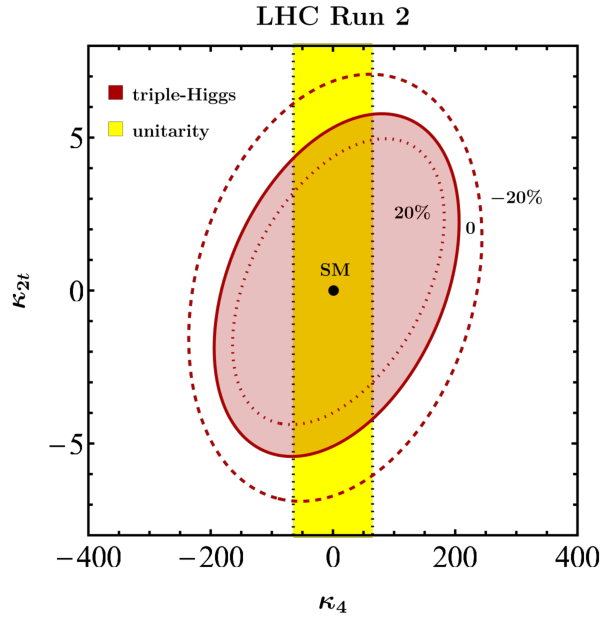
\includegraphics[width=0.45\textwidth]{LHCRun2_k4k2t_3h_YR5.pdf} \quad
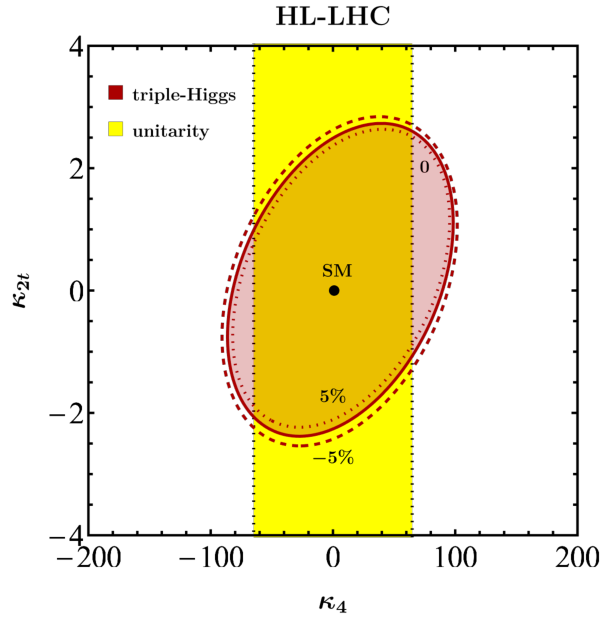
\includegraphics[width=0.45\textwidth]{HLLHC_k4k2t_3h_YR5.pdf}
\end{center}
\vspace{-4mm}
\caption{\label{fig:planes3} As \DIFaddbeginFL \DIFaddFL{in~}\DIFaddendFL Figure~\ref{fig:planes}, but in the $\kappa_4\hspace{0.25mm}$--$\hspace{0.25mm}\kappa_{2t}$ plane at LHC~Run~2~(left) and the HL-LHC~(right). The remaining parameters are fixed to their SM values, i.e.~\DIFdelbeginFL \DIFdelFL{$\kappa_3=1$ }\DIFdelendFL \DIFaddbeginFL \DIFaddFL{$\kappa_3=\kappa_t=1$ }\DIFaddendFL and \DIFdelbeginFL \DIFdelFL{$\kappa_t=1$}\DIFdelendFL \DIFaddbeginFL \DIFaddFL{$\kappa_{3t}=0$}\DIFaddendFL .}
\end{figure}

The two panels in~Figure~\ref{fig:planes} illustrate the \DIFdelbegin \DIFdel{expected }\DIFdelend sensitivity to the Higgs \DIFaddbegin \DIFadd{boson }\DIFaddend self-couplings~$\kappa_3$ and~$\kappa_4$ using \DIFdelbegin \DIFdel{current }\DIFdelend \DIFaddbegin \DIFadd{the full }\DIFaddend LHC~Run~2 data \DIFaddbegin \DIFadd{set }\DIFaddend and HL-LHC projections \DIFdelbegin \DIFdel{, assuming an integrated luminosity of }\DIFdelend \DIFaddbegin \DIFadd{corresponding to }\DIFaddend $3\,\mathrm{ab}^{-1}$ \DIFaddbegin \DIFadd{per experiment}\DIFaddend . The red contours indicate the $95\%$~CL constraints derived from \DIFdelbegin \DIFdel{triple-Higgs }\DIFdelend \DIFaddbegin \DIFadd{triple-Higgs-boson }\DIFaddend production in gluon fusion using the \DIFdelbegin \DIFdel{parameterisations }\DIFdelend \DIFaddbegin \DIFadd{parametrisations }\DIFaddend in~Eqs.~(\ref{eq:c00_13})\DIFdelbegin \DIFdel{to~}\DIFdelend \DIFaddbegin \DIFadd{--}\DIFaddend (\ref{eq:c40_13}) and~Eqs.~(\ref{eq:c00_14})\DIFdelbegin \DIFdel{to~}\DIFdelend \DIFaddbegin \DIFadd{--}\DIFaddend (\ref{eq:c40_14}), with the normalisation to the corresponding LO SM cross section given in~Eq.~(\ref{eq:SMLO}). For LHC~Run~2, the \DIFdelbegin \DIFdel{triple-Higgs }\DIFdelend \DIFaddbegin \DIFadd{triple-Higgs-boson }\DIFaddend constraints are obtained by imposing $\mu_{3h}^{\text{LHC~Run~2}} < 588$~\cite{CMS-PAS-HIG-24-012}, while for the HL-LHC we assume a projected upper limit of $\mu_{3h}^{\text{HL-LHC}} < 125$~\cite{ATL-PHYS-PUB-2025-003}. Throughout this analysis, we set \DIFdelbegin \DIFdel{$\kappa_{2t}=0$}\DIFdelend \DIFaddbegin \DIFadd{$\kappa_{2t}=\kappa_{3t}=0$}\DIFaddend , and the black \DIFdelbegin \DIFdel{dots }\DIFdelend \DIFaddbegin \DIFadd{points }\DIFaddend indicate the SM prediction. The left panel demonstrates that modifications of the top-quark Yukawa coupling of $\Delta\kappa_t=\pm20\%$, where $\Delta\kappa_t=\kappa_t-1$, which remain allowed at \DIFdelbegin \DIFdel{the }\DIFdelend $95\%$~CL after LHC~Run~2~\cite{ATLAS:2022vkf,CMS:2022dwd}, have a significant impact on the resulting constraints. This behaviour was already pointed out in~Ref.~\cite{Panizzi:2025sya} and originates from the strong power-law dependence of the coefficients $c_{nm}^{\sqrt{s}}\!\left(\kappa_t,\kappa_{2t}\right)$ appearing in~Eqs.~(\ref{eq:c00_13})\DIFdelbegin \DIFdel{to~}\DIFdelend \DIFaddbegin \DIFadd{--}\DIFaddend (\ref{eq:c40_14}) on $\kappa_t$. By the end of the HL-LHC, the top-quark Yukawa coupling is expected to be measured with a precision of $\Delta\kappa_t=\pm5\%$ at \DIFdelbegin \DIFdel{the }\DIFdelend $95\%$~CL~\cite{ATL-PHYS-PUB-2025-018}. Consequently, its impact on the $gg\to3h$ constraints in the $\kappa_3$--$\kappa_4$ plane will be substantially reduced, as illustrated in the right panel. Finally, we note that the projected HL-LHC constraints from $gg\to3h$ are comparable to those imposed by perturbative unitarity~\cite{Liu:2018peg,Stylianou:2023xit,DiLuzio:2017tfn}, shown as the yellow region enclosed by the black-dotted contour in both panels.

The panels in~Figures~\ref{fig:planes2} and~\ref{fig:planes3} show the expected sensitivity in the $\kappa_3\hspace{0.25mm}$--$\hspace{0.25mm}\kappa_{2t}$ and $\kappa_4\hspace{0.25mm}$--$\hspace{0.25mm}\kappa_{2t}$ planes, respectively. The red contours represent the $95\%$~CL constraints from \DIFdelbegin \DIFdel{triple-Higgs }\DIFdelend \DIFaddbegin \DIFadd{triple-Higgs-boson }\DIFaddend production in gluon fusion, obtained following the procedure described above. Parameters not shown explicitly are fixed to their SM values, and the black \DIFdelbegin \DIFdel{dots }\DIFdelend \DIFaddbegin \DIFadd{points }\DIFaddend indicate the SM prediction. As~in~Figure~\ref{fig:planes}, the left panels demonstrate that variations of the top-quark Yukawa coupling of $\Delta\kappa_t=\pm20\%$ can have a significant impact on the resulting constraints, whereas the smaller variations $\Delta\kappa_t=\pm5\%$ considered in the right panels lead to only minor changes. For $\kappa_{2t}$, \DIFdelbegin \DIFdel{triple-Higgs }\DIFdelend \DIFaddbegin \DIFadd{triple-Higgs-boson }\DIFaddend production at LHC~Run~2 yields $-5.1 < \kappa_{2t} < 5.3$, while the HL-LHC is expected to improve this range to $-2.3 < \kappa_{2t} < 2.5$ at $95\%$~CL. These limits are obtained by fixing $\kappa_3=\kappa_4=\kappa_t=1$ \DIFaddbegin \DIFadd{and $\kappa_{3t}=0$}\DIFaddend . We note that, under the same assumptions, the $95\%$~CL constraint on the \DIFdelbegin \DIFdel{double-Higgs }\DIFdelend \DIFaddbegin \DIFadd{double-Higgs-boson }\DIFaddend production signal strength obtained at LHC~Run~2, $\mu_{2h}^{\text{LHC~Run~2}}<2.5$~\cite{CMS:2026nuu}, already implies $-0.19 < \kappa_{2t} < 0.72$. The quoted bound is obtained using the expressions given in~Refs.~\cite{Buchalla:2018yce,Brivio:2025sib}. Consequently, \DIFdelbegin \DIFdel{triple-Higgs }\DIFdelend \DIFaddbegin \DIFadd{triple-Higgs-boson }\DIFaddend production is not expected to provide a stronger constraint on $\kappa_{2t}$ than \DIFdelbegin \DIFdel{double-Higgs }\DIFdelend \DIFaddbegin \DIFadd{double-Higgs-boson }\DIFaddend production in a single-parameter analysis. It~can, however, provide complementary information in multi-parameter fits, in particular when these involve~$\kappa_4$, which can only be weakly constrained by \DIFdelbegin \DIFdel{double-Higgs }\DIFdelend \DIFaddbegin \DIFadd{double-Higgs-boson }\DIFaddend production~\cite{Bizon:2018syu,Borowka:2018pxx,Li:2024iio,Ding:2026qto}.

\DIFaddbegin \subsection{\boldmath{Including the two-top--three-Higgs-boson interaction}}
\label{sec:kappa3t}

\DIFadd{We next extend the inclusive-rate parametrisation to the contact interaction between two top quarks and three Higgs bosons in~Eq.~(\ref{eq:Lkappa}). We generate loop-induced LO parton-level samples with \texttt{MadGraph5\_aMC@NLO}~\cite{Alwall:2014hca}, using the same Higgs boson mass $m_h$, top-quark mass $m_t$, PDFs, and scale choice as above. In this scan, $\kappa_t=1$ and $\kappa_{2t}=0$ are fixed.
}

\DIFadd{Following Eq.~(\ref{eq:BSMLO}), we write the extended cross section as
}\beq \label{eq:BSMLO3t}
\DIFadd{\sigma_{\mathrm{LO}}^{\sqrt{s}} = }\big(\DIFadd{\sigma_{\mathrm{LO}}^{\sqrt{s}}}\big)\DIFadd{_{\mathrm{SM}}
\sum_{n,m} c_{nm}^{\sqrt{s}}\!}\left(\DIFadd{\kappa_{3t}}\right)
\big(\DIFadd{\Delta\kappa_3}\big)\DIFadd{^n }\big(\DIFadd{\Delta\kappa_4}\big)\DIFadd{^m\,.
}\eeq
\DIFadd{This is an exact regrouping of the LO coupling basis at the fixed values $\kappa_t=1$ and $\kappa_{2t}=0$. Since the amplitude is linear in $\kappa_{3t}$, $c_{00}$ is at most quadratic in $\kappa_{3t}$, while $c_{01}$, $c_{10}$, and $c_{20}$ are at most linear; the remaining nonzero coefficient functions are constant. The fitted SM cross sections are
}\beq \label{eq:SMLO3t}
\big(\DIFadd{\sigma_{\mathrm{LO}}^{13\,\mathrm{TeV}}}\big)\DIFadd{_{\mathrm{SM}} = 42.12\,\mathrm{ab}\,,}\qquad
\big(\DIFadd{\sigma_{\mathrm{LO}}^{13.6\,\mathrm{TeV}}}\big)\DIFadd{_{\mathrm{SM}} = 47.40\,\mathrm{ab}\,,}\qquad
\big(\DIFadd{\sigma_{\mathrm{LO}}^{14\,\mathrm{TeV}}}\big)\DIFadd{_{\mathrm{SM}} = 51.08\,\mathrm{ab}\,.
}\eeq
\DIFadd{They agree to within $1.1\%$ with the independent values in~Eq.~(\ref{eq:SMLO}).
}

\DIFadd{The normalisation fixes $c_{00}^{\sqrt{s}}(0)=1$. The fitted coefficient functions are listed below. Their additional decimal places, compared with the first parametrisation, are retained to reproduce the numerical accuracy of the fit.
}

\DIFadd{For $\sqrt{s}=13\,\mathrm{TeV}$, the non-vanishing coefficient functions are
}\begin{align}
\DIFadd{c_{00}^{13\,\mathrm{TeV}}(\kappa_{3t}) }&\DIFadd{= 1-2.83183\,\kappa_{3t}+15.81829\,\kappa_{3t}^{2}\,, }\\
\DIFadd{c_{01}^{13\,\mathrm{TeV}}(\kappa_{3t}) }&\DIFadd{= -0.0914560+0.793591\,\kappa_{3t}\,, }\\
\DIFadd{c_{02}^{13\,\mathrm{TeV}}(\kappa_{3t}) }&\DIFadd{= 0.0168979\,, }\\
\DIFadd{c_{10}^{13\,\mathrm{TeV}}(\kappa_{3t}) }&\DIFadd{= -0.865038-3.92841\,\kappa_{3t}\,, }\\
\DIFadd{c_{11}^{13\,\mathrm{TeV}}(\kappa_{3t}) }&\DIFadd{= -0.167158\,, }\\
\DIFadd{c_{20}^{13\,\mathrm{TeV}}(\kappa_{3t}) }&\DIFadd{= 0.872294+0.900894\,\kappa_{3t}\,, }\\
\DIFadd{c_{21}^{13\,\mathrm{TeV}}(\kappa_{3t}) }&\DIFadd{= 0.0487935\,, }\\
\DIFadd{c_{30}^{13\,\mathrm{TeV}}(\kappa_{3t}) }&\DIFadd{= -0.259375\,, }\\
\DIFadd{c_{40}^{13\,\mathrm{TeV}}(\kappa_{3t}) }&\DIFadd{= 0.0395354\,.
}\end{align}
\DIFadd{For $\sqrt{s}=13.6\,\mathrm{TeV}$, they are
}\begin{align}
\DIFadd{c_{00}^{13.6\,\mathrm{TeV}}(\kappa_{3t}) }&\DIFadd{= 1-2.87872\,\kappa_{3t}+16.21306\,\kappa_{3t}^{2}\,, }\\
\DIFadd{c_{01}^{13.6\,\mathrm{TeV}}(\kappa_{3t}) }&\DIFadd{= -0.0909154+0.800038\,\kappa_{3t}\,, }\\
\DIFadd{c_{02}^{13.6\,\mathrm{TeV}}(\kappa_{3t}) }&\DIFadd{= 0.0168638\,, }\\
\DIFadd{c_{10}^{13.6\,\mathrm{TeV}}(\kappa_{3t}) }&\DIFadd{= -0.866564-3.95165\,\kappa_{3t}\,, }\\
\DIFadd{c_{11}^{13.6\,\mathrm{TeV}}(\kappa_{3t}) }&\DIFadd{= -0.166501\,, }\\
\DIFadd{c_{20}^{13.6\,\mathrm{TeV}}(\kappa_{3t}) }&\DIFadd{= 0.871502+0.897150\,\kappa_{3t}\,, }\\
\DIFadd{c_{21}^{13.6\,\mathrm{TeV}}(\kappa_{3t}) }&\DIFadd{= 0.0485042\,, }\\
\DIFadd{c_{30}^{13.6\,\mathrm{TeV}}(\kappa_{3t}) }&\DIFadd{= -0.257216\,, }\\
\DIFadd{c_{40}^{13.6\,\mathrm{TeV}}(\kappa_{3t}) }&\DIFadd{= 0.0390715\,.
}\end{align}
\DIFadd{For $\sqrt{s}=14\,\mathrm{TeV}$, they are
}\begin{align}
\DIFadd{c_{00}^{14\,\mathrm{TeV}}(\kappa_{3t}) }&\DIFadd{= 1-2.95187\,\kappa_{3t}+16.47338\,\kappa_{3t}^{2}\,, }\\
\DIFadd{c_{01}^{14\,\mathrm{TeV}}(\kappa_{3t}) }&\DIFadd{= -0.0921387+0.803365\,\kappa_{3t}\,, }\\
\DIFadd{c_{02}^{14\,\mathrm{TeV}}(\kappa_{3t}) }&\DIFadd{= 0.0168553\,, }\\
\DIFadd{c_{10}^{14\,\mathrm{TeV}}(\kappa_{3t}) }&\DIFadd{= -0.853992-3.93891\,\kappa_{3t}\,, }\\
\DIFadd{c_{11}^{14\,\mathrm{TeV}}(\kappa_{3t}) }&\DIFadd{= -0.166145\,, }\\
\DIFadd{c_{20}^{14\,\mathrm{TeV}}(\kappa_{3t}) }&\DIFadd{= 0.863440+0.899872\,\kappa_{3t}\,, }\\
\DIFadd{c_{21}^{14\,\mathrm{TeV}}(\kappa_{3t}) }&\DIFadd{= 0.0482948\,, }\\
\DIFadd{c_{30}^{14\,\mathrm{TeV}}(\kappa_{3t}) }&\DIFadd{= -0.255934\,, }\\
\DIFadd{c_{40}^{14\,\mathrm{TeV}}(\kappa_{3t}) }&\DIFadd{= 0.0390078\,.
}\end{align}


\clearpage

\begin{figure}[t!]
\begin{center}
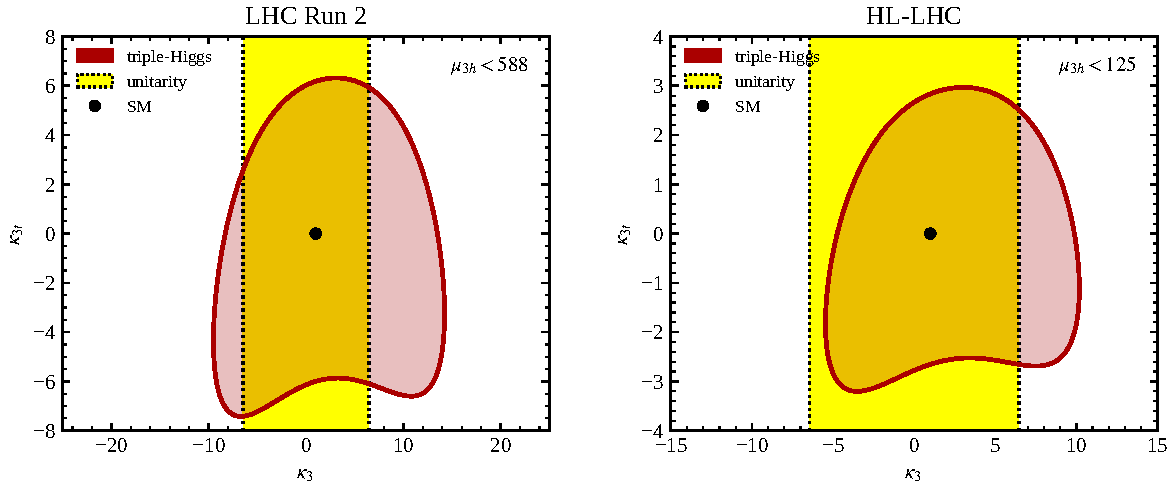
\includegraphics[width=0.96\textwidth]{ct3-k3-k3t-constraints.pdf}
\end{center}
\vspace{-4mm}
\caption{\label{fig:planes3t_k3} \DIFaddFL{Constraints in the $\kappa_3\hspace{0.25mm}$--$\hspace{0.25mm}\kappa_{3t}$ plane at LHC~Run~2~(left) and the HL-LHC~(right), obtained from Eq.~(\ref{eq:BSMLO3t}) using $\mu_{3h}<588$ and $\mu_{3h}<125$, respectively. The red regions are allowed by the inclusive triple-Higgs-boson rate, the black points denote the SM, and the yellow vertical bands show the projection of the tree-level $hh\to hh$ perturbative-unitarity constraint. We fix $\kappa_4=\kappa_t=1$ and $\kappa_{2t}=0$. The yellow band constrains $\kappa_3$ only; no independent unitarity condition on $\kappa_{3t}$ is imposed.}}
\end{figure}

\begin{figure}[t!]
\begin{center}
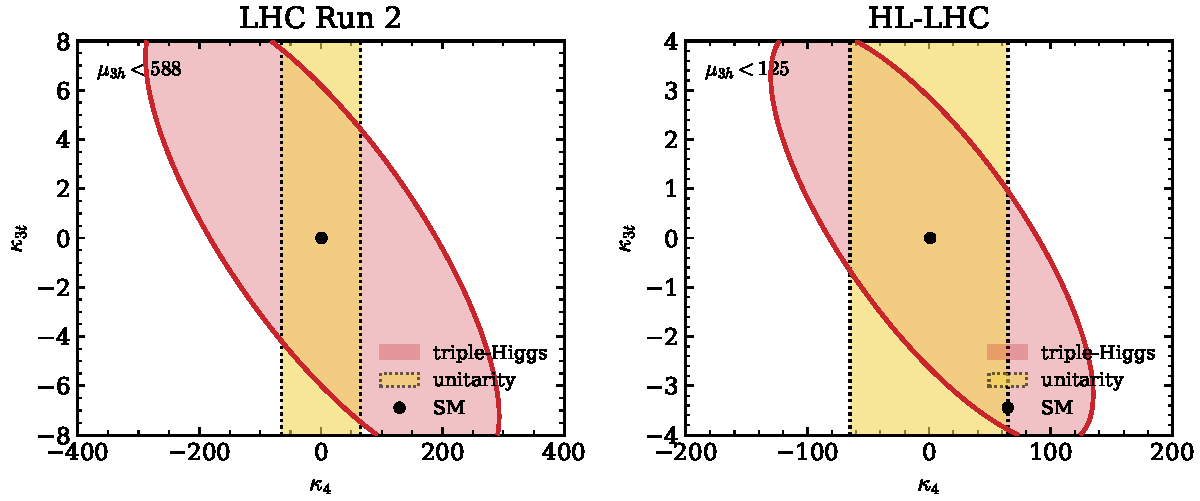
\includegraphics[width=0.96\textwidth]{ct3-k4-k3t-constraints.pdf}
\end{center}
\vspace{-4mm}
\caption{\label{fig:planes3t_k4} \DIFaddFL{As in~Figure~\ref{fig:planes3t_k3}, but in the $\kappa_4\hspace{0.25mm}$--$\hspace{0.25mm}\kappa_{3t}$ plane with $\kappa_3=\kappa_t=1$ and $\kappa_{2t}=0$. The yellow band is the projection of the $hh\to hh$ perturbative-unitarity condition onto $\kappa_4$.}}
\end{figure}

\DIFadd{Figures~\ref{fig:planes3t_k3} and~\ref{fig:planes3t_k4} are the $\kappa_{3t}$ analogues of Figures~\ref{fig:planes2} and~\ref{fig:planes3}. Fixing all other couplings to their SM values yields
}\beq
\DIFadd{-6.00<\kappa_{3t}<6.18}\qquad\DIFadd{(\text{LHC Run 2})\,,
}\qquad
\DIFadd{-2.66<\kappa_{3t}<2.83}\qquad\DIFadd{(\text{HL-LHC})\,.
}\eeq
\DIFadd{The quadratic form also exposes an inclusive-rate degeneracy. At $\kappa_3=\kappa_4=1$, the two solutions of $c_{00}^{\sqrt{s}}(\kappa_{3t})=1$ are $\kappa_{3t}=0$ and an energy-dependent second solution near $\kappa_{3t}=0.179$. Differential information is therefore essential for distinguishing these two solutions.
}

\DIFaddend \begin{figure}[t!]
\begin{center}
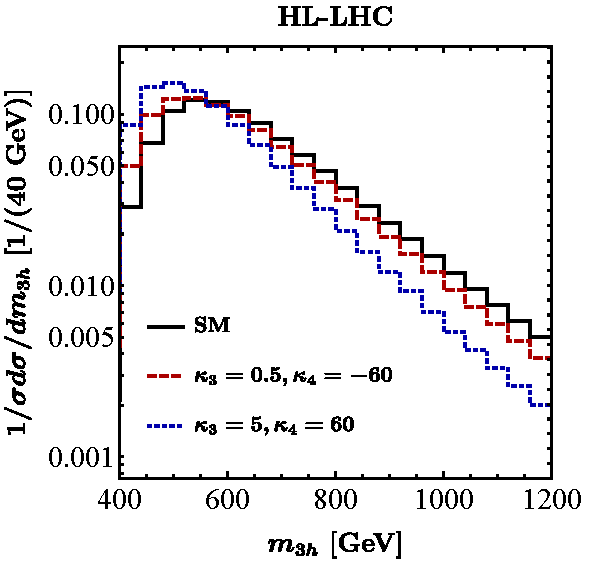
\includegraphics[width=0.45\textwidth]{HLLHC_m3h_uni_YR5.pdf} \quad
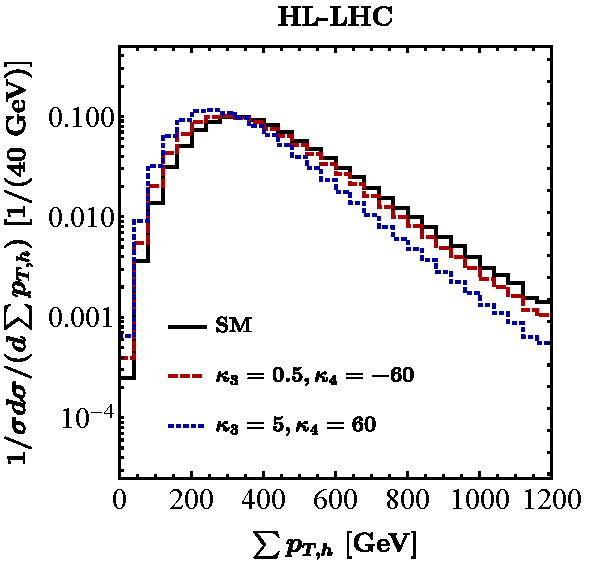
\includegraphics[width=0.45\textwidth]{HLLHC_sum_pTh_uni_YR5.pdf}
\end{center}
\vspace{-2mm}
\caption{\label{fig:distributions} Normalised kinematic distributions for $gg \to 3h$ production at the HL-LHC in the SM~(solid black line) and in two benchmark scenarios defined by $\kappa_3$ and~$\kappa_4$~(red dashed and blue dotted lines). The left and right panels show the invariant mass of the \DIFdelbeginFL \DIFdelFL{three-Higgs }\DIFdelendFL \DIFaddbeginFL \DIFaddFL{three-Higgs-boson }\DIFaddendFL system, $m_{3h}$, and the scalar sum of the transverse momenta of the Higgs bosons, $\textstyle\sum p_{T,h}$, respectively. All results are obtained for $\kappa_t=1$ and \DIFdelbeginFL \DIFdelFL{$\kappa_{2t}=0$}\DIFdelendFL \DIFaddbeginFL \DIFaddFL{$\kappa_{2t}=\kappa_{3t}=0$}\DIFaddendFL .}
\end{figure}

Modifications of the Higgs \DIFaddbegin \DIFadd{boson }\DIFaddend trilinear and quartic self-couplings affect \DIFdelbegin \DIFdel{not only the inclusive triple-Higgs production cross section but also }\DIFdelend \DIFaddbegin \DIFadd{both the inclusive $gg\to3h$ cross section and }\DIFaddend the kinematic properties of the \DIFdelbegin \DIFdel{$gg \to 3h$ }\DIFdelend final state. \DIFdelbegin \DIFdel{To illustrate this point, }\DIFdelend Figure~\ref{fig:distributions} \DIFdelbegin \DIFdel{shows normalised kinematic distributions at the HL-LHC }\DIFdelend \DIFaddbegin \DIFadd{compares normalised distributions }\DIFaddend for the SM \DIFdelbegin \DIFdel{and two BSM benchmark scenarios. Both benchmark points yield the same inclusive signal strength, $\mu_{3h}=65$, with }\DIFdelend \DIFaddbegin \DIFadd{with two BSM benchmarks. Both benchmarks give $\mu_{3h}\simeq65$, and their }\DIFaddend inclusive cross sections \DIFdelbegin \DIFdel{differing by only about }\DIFdelend \DIFaddbegin \DIFadd{differ by less than }\DIFaddend $5\%$, while \DIFdelbegin \DIFdel{remaining consistent with the perturbative unitarity bounds obtained }\DIFdelend \DIFaddbegin \DIFadd{their values of $\kappa_3$ and $\kappa_4$ satisfy the perturbative-unitarity constraints }\DIFaddend from tree-level \DIFdelbegin \DIFdel{$hh \to hh$ scattering. The left and right panels show the invariant mass of the three-Higgs system, $m_{3h}$, and the scalar sum of the Higgs transverse momenta, $\textstyle\sum p_{T,h}$, respectively. All~results are obtained for }\DIFdelend \DIFaddbegin \DIFadd{$hh\to hh$ scattering. We set }\DIFaddend $\kappa_t=1$ and \DIFdelbegin \DIFdel{$\kappa_{2t}=0$. This choice is motivated by the observation of~Ref. ~\cite{Panizzi:2025sya} that variations }\DIFdelend \DIFaddbegin \DIFadd{$\kappa_{2t}=\kappa_{3t}=0$. Variations }\DIFaddend of $\kappa_t$ \DIFdelbegin \DIFdel{approximately induce an overall rescaling of the normalised distributions, without significantly altering their shapes. The comparison demonstrates that values of $\kappa_3$ and $\kappa_4$ yielding nearly degenerate inclusive cross sections can nevertheless lead to sizeable distortions of the differential spectra, reaching }\DIFdelend \DIFaddbegin \DIFadd{predominantly rescale the unnormalised spectra and therefore have little effect on their normalised shapes~\cite{Panizzi:2025sya}. Nevertheless, the two benchmarks produce deviations of }\DIFaddend up to about $50\%$ in \DIFdelbegin \DIFdel{both the $m_{3h}$ and ~$\textstyle\sum p_{T,h}$ distributions, in }\DIFdelend the peak regions \DIFdelbegin \DIFdel{as well as in the }\DIFdelend \DIFaddbegin \DIFadd{and }\DIFaddend high-energy tails \DIFdelbegin \DIFdel{. Consequently, exploiting differential information in }\DIFdelend \DIFaddbegin \DIFadd{of both distributions. Differential information can therefore strengthen }\DIFaddend future HL-LHC \DIFdelbegin \DIFdel{analyses of $gg \to 3h$ production has the potential to improve the constraint quoted below }\DIFdelend \DIFaddbegin \DIFadd{constraints beyond the projected interval in~}\DIFaddend Eq.~(\DIFdelbegin \DIFdel{\ref{eq:kappa4bounds}}\DIFdelend \DIFaddbegin \DIFadd{\ref{eq:kappa4boundsHL}}\DIFaddend ), which \DIFdelbegin \DIFdel{currently relies on the inclusive ~rate ~only}\DIFdelend \DIFaddbegin \DIFadd{is obtained from the inclusive rate alone}\DIFaddend ~\cite{Ding:2026qto}.

\begin{figure}[t!]
\begin{center}
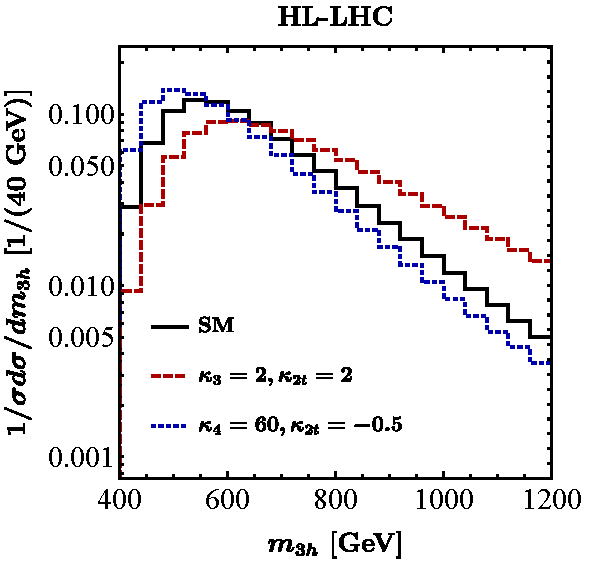
\includegraphics[width=0.45\textwidth]{HLLHC_k2t_m3h_uni_YR5.pdf} \quad
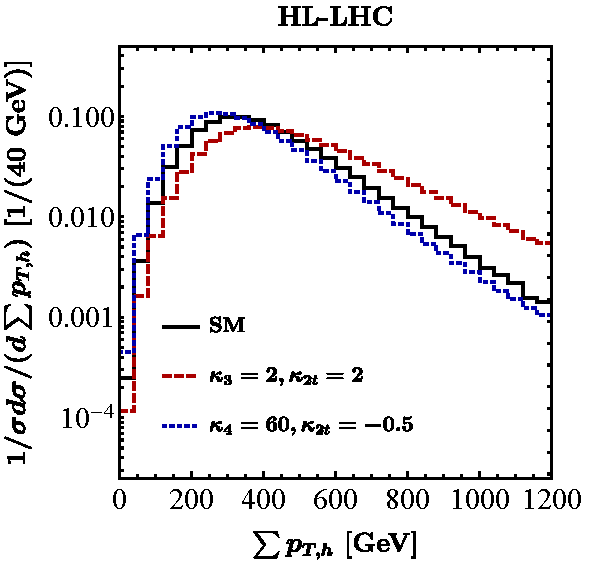
\includegraphics[width=0.45\textwidth]{HLLHC_k2t_sum_pTh_uni_YR5.pdf}
\end{center}
\vspace{-2mm}
\caption{\label{fig:distributions2} As in~Figure~\ref{fig:distributions}, but for two \DIFdelbeginFL \DIFdelFL{other $\kappa$-benchmark }\DIFdelendFL \DIFaddbeginFL \DIFaddFL{further benchmark }\DIFaddendFL scenarios \DIFaddbeginFL \DIFaddFL{in the $\kappa$-framework, as }\DIFaddendFL indicated in the panels. The remaining parameters are fixed to their SM values\DIFaddbeginFL \DIFaddFL{, including $\kappa_{3t}=0$}\DIFaddendFL .
}
\end{figure}

Figure~\ref{fig:distributions2} presents \DIFdelbegin \DIFdel{additional normalised kinematic distributions at the HL-LHC }\DIFdelend \DIFaddbegin \DIFadd{further normalised distributions }\DIFaddend for the SM and two \DIFdelbegin \DIFdel{further BSM benchmark scenarios within }\DIFdelend \DIFaddbegin \DIFadd{BSM benchmarks in }\DIFaddend the $\kappa$-framework. \DIFdelbegin \DIFdel{The benchmark points are selected such that both lead to an enhanced signal strength of $\mu_{3h}=75$, while }\DIFdelend \DIFaddbegin \DIFadd{Both benchmarks give $\mu_{3h}\simeq75$, and }\DIFaddend their inclusive cross sections differ by less than \DIFdelbegin \DIFdel{about }\DIFdelend $5\%$. The \DIFdelbegin \DIFdel{corresponding }\DIFdelend \DIFaddbegin \DIFadd{non-SM }\DIFaddend values of $\kappa_3$ \DIFdelbegin \DIFdel{and }\DIFdelend \DIFaddbegin \DIFadd{or }\DIFaddend $\kappa_4$ \DIFdelbegin \DIFdel{are consistent with perturbative unitarity constraints, and all }\DIFdelend \DIFaddbegin \DIFadd{satisfy the relevant perturbative-unitarity constraints, while the }\DIFaddend remaining parameters are fixed to their SM values\DIFaddbegin \DIFadd{, including $\kappa_{3t}=0$}\DIFaddend . As in~Figure~\ref{fig:distributions}, sizeable \DIFdelbegin \DIFdel{distortions of the differential spectra arise }\DIFdelend \DIFaddbegin \DIFadd{shape distortions remain }\DIFaddend despite the near-degeneracy of the inclusive rates. This \DIFdelbegin \DIFdel{further demonstrates that exploiting differential information }\DIFdelend \DIFaddbegin \DIFadd{illustrates how differential information can help to resolve parameter degeneracies }\DIFaddend in future \DIFaddbegin \DIFadd{$gg\to3h$ searches at the }\DIFaddend HL-LHC\DIFdelbegin \DIFdel{searches for $gg \to 3h$ production can help lift parameter degeneracies within the $\kappa$-framework}\DIFdelend .

\DIFaddbegin \FloatBarrier

\begin{figure}[H]
\begin{center}
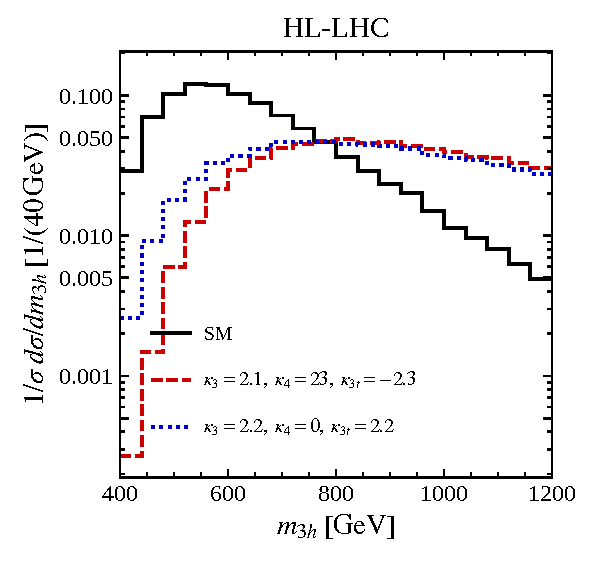
\includegraphics[width=0.45\textwidth]{14tev-ct3-mu65-benchmarks-m3h.pdf} \quad
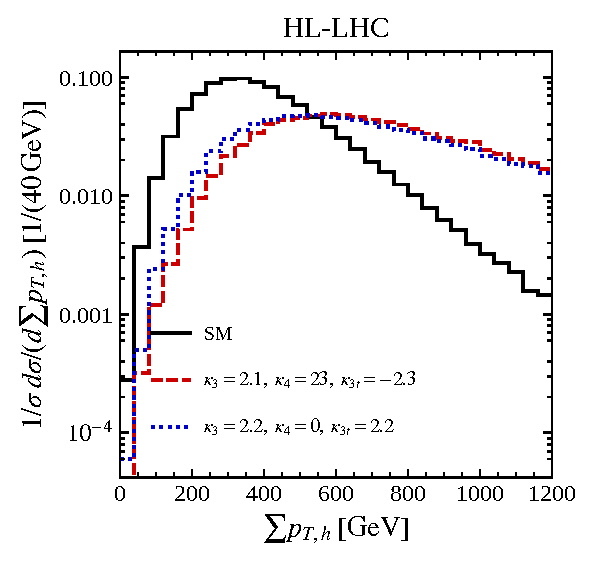
\includegraphics[width=0.45\textwidth]{14tev-ct3-mu65-benchmarks-sum-pth.pdf}
\end{center}
\vspace{-4mm}
\caption{\label{fig:ct3benchmarks} \DIFaddFL{Normalised $m_{3h}$ and $\sum p_{T,h}$ distributions at the HL-LHC for the SM and the two $\mu_{3h}\simeq65$ benchmarks $(\kappa_3,\kappa_4,\kappa_{3t})=(2.1,23,-2.3)$ and $(6.0,59,-0.50)$. The distributions use the same $40\,\mathrm{GeV}$ binning and plotting ranges as Figures~\ref{fig:distributions} and~\ref{fig:distributions2}. We fix $\kappa_t=1$ and $\kappa_{2t}=0$.}}
\end{figure}

\DIFadd{The two mixed-coupling benchmarks in~Figure~\ref{fig:ct3benchmarks} provide a particularly clear example of enhanced but nearly degenerate inclusive rates. Their $100\,000$-event samples give $\mu_{3h}=64.95$ and $64.80$, respectively, so their inclusive cross sections differ by only $0.24\%$. Nevertheless, their normalised distributions differ substantially from both the SM and one another. The $(2.1,23,-2.3)$ benchmark shifts weight towards larger invariant masses and transverse momenta, whereas the $(6.0,59,-0.50)$ benchmark enhances the near-threshold and low-$p_T$ regions. The samples use the same PDFs and scale choice as the inclusive-rate parametrisation.
}

\FloatBarrier

\DIFaddend \section{\textbf{\boldmath{Conclusions}}}
\label{sec:conclusions}

Unlike the Higgs \DIFaddbegin \DIFadd{boson }\DIFaddend couplings to EW gauge bosons and third-generation fermions, which are already being measured with increasing precision, the Higgs \DIFaddbegin \DIFadd{boson }\DIFaddend self-interactions remain largely unconstrained by LHC~Run~2 data. This leaves considerable room for BSM scenarios that modify the shape of the Higgs potential. Indeed, both theoretical considerations and explicit ultraviolet-complete constructions demonstrate that deviations of the Higgs \DIFaddbegin \DIFadd{boson }\DIFaddend self-couplings exceeding $200\%$ can be consistent with existing \DIFdelbegin \DIFdel{single-Higgs }\DIFdelend \DIFaddbegin \DIFadd{single-Higgs-boson }\DIFaddend measurements without requiring fine-tuned parameter choices~\cite{Durieux:2022hbu}. Measurements of \DIFdelbegin \DIFdel{multi-Higgs }\DIFdelend \DIFaddbegin \DIFadd{multi-Higgs-boson }\DIFaddend production at the HL-LHC and future colliders therefore provide a unique opportunity to probe largely unexplored regions of parameter space and \DIFdelbegin \DIFdel{retain }\DIFdelend \DIFaddbegin \DIFadd{offer }\DIFaddend significant discovery potential, even in scenarios where \DIFdelbegin \DIFdel{single-Higgs }\DIFdelend \DIFaddbegin \DIFadd{single-Higgs-boson }\DIFaddend observables remain close to their SM predictions.

In this note, we have derived compact \DIFdelbegin \DIFdel{``pocket formulas'' for triple-Higgs }\DIFdelend \DIFaddbegin \DIFadd{`pocket formulae' for triple-Higgs-boson }\DIFaddend production within the $\kappa$-framework, enabling constraints on the Higgs \DIFaddbegin \DIFadd{boson }\DIFaddend trilinear and quartic self-couplings to be obtained from current and future measurements of the $gg \to 3h$ signal strength. The \DIFdelbegin \DIFdel{resulting parameterisations retain }\DIFdelend \DIFaddbegin \DIFadd{parametrisation in Eq.~(\ref{eq:BSMLO}) retains }\DIFaddend the full dependence on $\kappa_3$, $\kappa_4$, $\kappa_t$, and $\kappa_{2t}$ at LO in perturbation theory \DIFdelbegin \DIFdel{. Since their }\DIFdelend \DIFaddbegin \DIFadd{for $\kappa_{3t}=0$. We have supplemented it with Eq.~(\ref{eq:BSMLO3t}), which includes the complete LO dependence on $\kappa_{3t}$ for $\kappa_t=1$ and $\kappa_{2t}=0$ at $13$, $13.6$, and $14\,\mathrm{TeV}$. Since the }\DIFaddend derivation relies on \DIFdelbegin \DIFdel{the flexible and efficient }\DIFdelend \DIFaddbegin \DIFadd{flexible }\DIFaddend matrix-element \DIFdelbegin \DIFdel{implementation developed in~Ref.~\cite{Campbell:2025llb}, the extension of these formulas }\DIFdelend \DIFaddbegin \DIFadd{implementations, further extensions }\DIFaddend to incorporate additional coupling modifications --- such as those arising at next-to-leading order in \DIFdelbegin \DIFdel{the Higgs Effective Field Theory}\DIFdelend \DIFaddbegin \DIFadd{Higgs effective field theory}\DIFaddend ~\cite{Brivio:2025sib} --- \DIFdelbegin \DIFdel{is~}\DIFdelend \DIFaddbegin \DIFadd{are }\DIFaddend comparatively straightforward.

Using these \DIFdelbegin \DIFdel{parameterisations}\DIFdelend \DIFaddbegin \DIFadd{parametrisations}\DIFaddend , we have \DIFdelbegin \DIFdel{investigated the sensitivity to $\kappa_3$ and $\kappa_4$ using current and projected LHC data}\DIFdelend \DIFaddbegin \DIFadd{studied how current LHC data and HL-LHC projections constrain $\kappa_3$ and $\kappa_4$}\DIFaddend . We find that the presently allowed uncertainty in $\kappa_t$ can have a substantial impact on the constraints in the $\kappa_3\hspace{0.25mm}$--$\hspace{0.25mm}\kappa_4$ plane. This dependence is significantly reduced at the HL-LHC, where the expected percent-level precision of the top-quark Yukawa coupling measurement will strongly restrict the corresponding parameter space. For~$\kappa_{2t}$, which parametrises the interaction between two top quarks and two Higgs bosons, we find that \DIFdelbegin \DIFdel{triple-Higgs }\DIFdelend \DIFaddbegin \DIFadd{triple-Higgs-boson }\DIFaddend production is unlikely to provide stronger bounds than \DIFdelbegin \DIFdel{double-Higgs }\DIFdelend \DIFaddbegin \DIFadd{double-Higgs-boson }\DIFaddend production in a single-parameter analysis. Nevertheless, it can yield complementary information in global multi-parameter fits, especially once $\kappa_4$ is included, as this coupling remains only weakly constrained by \DIFdelbegin \DIFdel{double-Higgs }\DIFdelend \DIFaddbegin \DIFadd{double-Higgs-boson }\DIFaddend measurements~\cite{Bizon:2018syu,Borowka:2018pxx,Li:2024iio,Ding:2026qto}. \DIFaddbegin \DIFadd{In a single-parameter interpretation, the current and projected upper limits on the triple-Higgs-boson rate give $-6.00<\kappa_{3t}<6.18$ and $-2.66<\kappa_{3t}<2.83$, respectively. The energy-dependent nonzero solution near $\kappa_{3t}=0.179$ is rate-degenerate with the SM. }\DIFaddend We further demonstrate that \DIFdelbegin \DIFdel{parameter choices for $\kappa_3$ and $\kappa_4$ yielding nearly identical inclusive $gg \to 3h$ cross sections can still produce substantial differences in differential observables. Similar effects are observed for variations of $\kappa_{2t}$}\DIFdelend \DIFaddbegin \DIFadd{differential information lifts inclusive-rate degeneracies and identifies mixed $(\kappa_3,\kappa_4,\kappa_{3t})$ benchmarks with $\mu_{3h}\simeq65$ but substantially different kinematic distributions from the SM and from one another}\DIFaddend .

The projected HL-LHC sensitivity to $\kappa_4$ in a single-parameter analysis remains modest, with constraints reaching only $|\kappa_4|\lesssim 80$, comparable to those derived from \DIFdelbegin \DIFdel{perturbative unitarity }\DIFdelend \DIFaddbegin \DIFadd{perturbative-unitarity }\DIFaddend arguments~\cite{Liu:2018peg,Stylianou:2023xit,DiLuzio:2017tfn}. An improvement by approximately one order of magnitude in the determination of the Higgs \DIFaddbegin \DIFadd{boson }\DIFaddend quartic self-coupling could be achieved at \DIFdelbegin \DIFdel{a }\DIFdelend \DIFaddbegin \DIFadd{the proposed }\DIFaddend hadron-collider \DIFdelbegin \DIFdel{option }\DIFdelend \DIFaddbegin \DIFadd{stage }\DIFaddend of the Future Circular Collider~\cite{Papaefstathiou:2015paa,Chen:2015gva,Fuks:2015hna,Kilian:2017nio,Fuks:2017zkg,Bizon:2018syu,Papaefstathiou:2023uum,Abouabid:2024gms,Dong:2025lkm,Haisch:2025pql,Fuks:2025gjv}. Reaching a precision at the level of $50\%$, however, would likely require the capabilities of a future muon collider~\cite{Chiesa:2020awd}.

\section*{Acknowledgements}
UH acknowledges Konstantin Schmid for helpful discussions. This manuscript has been authored by Fermi Forward Discovery Group, LLC under Contract No. 89243024CSC000002 with the U.S.\ Department of Energy, Office of Science, Office of High Energy Physics. RKE~acknowledges receipt of a Leverhulme Emeritus Fellowship from the Leverhulme Trust.

%\bibliographystyle{JHEP}
%\bibliography{ref}

\begin{thebibliography}{10}
\providecommand{\url}[1]{\texttt{#1}}
\providecommand{\urlprefix}{URL }
\expandafter\ifx\csname urlstyle\endcsname\relax
  \providecommand{\doi}[1]{doi:\discretionary{}{}{}#1}\else
  \providecommand{\doi}{doi:\discretionary{}{}{}\begingroup \urlstyle{rm}\Url}\fi
\providecommand{\eprint}[2][]{\url{#2}}

\bibitem{ATLAS:2012yve}
G.~Aad \emph{et~al.},
\newblock \emph{{Observation of a new particle in the search for the Standard Model Higgs boson with the ATLAS detector at the LHC}},
\newblock Phys. Lett. B \textbf{716}, 1 (2012),
\newblock \doi{10.1016/j.physletb.2012.08.020},
\newblock \eprint{1207.7214}.

\bibitem{CMS:2012qbp}
S.~Chatrchyan \emph{et~al.},
\newblock \emph{{Observation of a New Boson at a Mass of 125~GeV with the CMS Experiment at the LHC}},
\newblock Phys. Lett. B \textbf{716}, 30 (2012),
\newblock \doi{10.1016/j.physletb.2012.08.021},
\newblock \eprint{1207.7235}.

\bibitem{DiMicco:2019ngk}
J.~Alison \emph{et~al.},
\newblock \emph{{Higgs boson potential at colliders: Status and perspectives}},
\newblock Rev. Phys. \textbf{5}, 100045 (2020),
\newblock \doi{10.1016/j.revip.2020.100045},
\newblock \eprint{1910.00012}.

\bibitem{Durieux:2022hbu}
G.~Durieux, M.~McCullough and E.~Salvioni,
\newblock \emph{{Charting the Higgs self-coupling boundaries}},
\newblock JHEP \textbf{12}, 148 (2022),
\newblock \doi{10.1007/JHEP12(2022)148},
\newblock [Erratum: JHEP {\bf 02}, 165 (2023)],
\newblock \eprint{2209.00666}.

\bibitem{Gorbahn:2016uoy}
M.~Gorbahn and U.~Haisch,
\newblock \emph{{Indirect probes of the trilinear Higgs coupling: $gg \to h$ and $h \to \gamma \gamma$}},
\newblock JHEP \textbf{10}, 094 (2016),
\newblock \doi{10.1007/JHEP10(2016)094},
\newblock \eprint{1607.03773}.

\bibitem{Degrassi:2016wml}
G.~Degrassi, P.~P. Giardino, F.~Maltoni and D.~Pagani,
\newblock \emph{{Probing the Higgs self coupling via single Higgs production at the LHC}},
\newblock JHEP \textbf{12}, 080 (2016),
\newblock \doi{10.1007/JHEP12(2016)080},
\newblock \eprint{1607.04251}.

\bibitem{Bizon:2016wgr}
W.~Bizon, M.~Gorbahn, U.~Haisch and G.~Zanderighi,
\newblock \emph{{Constraints on the trilinear Higgs coupling from vector boson fusion and associated Higgs production at the LHC}},
\newblock JHEP \textbf{07}, 083 (2017),
\newblock \doi{10.1007/JHEP07(2017)083},
\newblock \eprint{1610.05771}.

\bibitem{Maltoni:2017ims}
F.~Maltoni, D.~Pagani, A.~Shivaji and X.~Zhao,
\newblock \emph{{Trilinear Higgs coupling determination via single-Higgs differential measurements at the LHC}},
\newblock Eur. Phys. J. C \textbf{77}(12), 887 (2017),
\newblock \doi{10.1140/epjc/s10052-017-5410-8},
\newblock \eprint{1709.08649}.

\bibitem{Gorbahn:2019lwq}
M.~Gorbahn and U.~Haisch,
\newblock \emph{{Two-loop amplitudes for Higgs plus jet production involving a modified trilinear Higgs coupling}},
\newblock JHEP \textbf{04}, 062 (2019),
\newblock \doi{10.1007/JHEP04(2019)062},
\newblock \eprint{1902.05480}.

\bibitem{Haisch:2021hvy}
U.~Haisch and G.~Koole,
\newblock \emph{{Off-shell Higgs production at the LHC as a probe of the trilinear Higgs coupling}},
\newblock JHEP \textbf{02}, 030 (2022),
\newblock \doi{10.1007/JHEP02(2022)030},
\newblock \eprint{2111.12589}.

\bibitem{Gao:2023bll}
J.~Gao, X.-M. Shen, G.~Wang, L.~L. Yang and B.~Zhou,
\newblock \emph{{Probing the Higgs boson trilinear self-coupling through Higgs boson+jet production}},
\newblock Phys. Rev. D \textbf{107}(11), 115017 (2023),
\newblock \doi{10.1103/PhysRevD.107.115017},
\newblock \eprint{2302.04160}.

\bibitem{Haisch:2024nzv}
U.~Haisch and M.~Niggetiedt,
\newblock \emph{{Exact two-loop amplitudes for Higgs plus jet production with a cubic Higgs self-coupling}},
\newblock JHEP \textbf{10}, 236 (2024),
\newblock \doi{10.1007/JHEP10(2024)236},
\newblock \eprint{2408.13186}.

\bibitem{Ghosh:2025fma}
A.~Ghosh, M.~Griese, U.~Haisch and T.~H. Park,
\newblock \emph{{Neural simulation-based inference of the Higgs trilinear self-coupling via off-shell Higgs production}},
\newblock Eur. Phys. J. C \textbf{86}(4), 415 (2026),
\newblock \doi{10.1140/epjc/s10052-026-15605-3},
\newblock \eprint{2507.02032}.

\bibitem{LHCHiggsCrossSectionWorkingGroup:2012nn}
A.~David, A.~Denner, M.~Duehrssen, M.~Grazzini, C.~Grojean, G.~Passarino, M.~Schumacher, M.~Spira, G.~Weiglein and M.~Zanetti,
\newblock \emph{{LHC HXSWG interim recommendations to explore the coupling structure of a Higgs-like particle}}  (2012),
\newblock \eprint{1209.0040}.

\bibitem{LHCHiggsCrossSectionWorkingGroup:2013rie}
J.~R. Andersen \emph{et~al.},
\newblock \emph{{Handbook of LHC Higgs Cross Sections: 3. Higgs Properties}}  (2013),
\newblock \doi{10.5170/CERN-2013-004},
\newblock \eprint{1307.1347}.

\bibitem{LHCHiggsCrossSectionWorkingGroup:2016ypw}
D.~de~Florian \emph{et~al.},
\newblock \emph{{Handbook of LHC Higgs Cross Sections: 4. Deciphering the Nature of the Higgs Sector}},
\newblock CERN Yellow Rep. Monogr. \textbf{2}, 1 (2017),
\newblock \doi{10.23731/CYRM-2017-002},
\newblock \eprint{1610.07922}.

\bibitem{CMS:2026nuu}
G.~Aad \emph{et~al.},
\newblock \emph{{Combination of ATLAS and CMS searches for Higgs boson pair production at $\sqrt{s}$~=~13~TeV}}  (2026),
\newblock \eprint{2602.23991}.

\bibitem{deFlorian:2019app}
D.~de~Florian, I.~Fabre and J.~Mazzitelli,
\newblock \emph{{Triple Higgs production at hadron colliders at NNLO in QCD}},
\newblock JHEP \textbf{03}, 155 (2020),
\newblock \doi{10.1007/JHEP03(2020)155},
\newblock \eprint{1912.02760}.

\bibitem{ATLAS:2024xcs}
G.~Aad \emph{et~al.},
\newblock \emph{{Search for triple Higgs boson production in the 6b final state using pp collisions at $\sqrt{s}$~=~13~TeV with the ATLAS detector}},
\newblock Phys. Rev. D \textbf{111}(3), 032006 (2025),
\newblock \doi{10.1103/PhysRevD.111.032006},
\newblock \eprint{2411.02040}.

\bibitem{CMS-PAS-HIG-24-012}
\emph{{Search for nonresonant triple Higgs boson production in the six b-quark final state in proton-proton collisions at 13~TeV}},
\newblock CERN, Geneva (2025),
\newblock \href{https://cds.cern.ch/record/2945361}{https://cds.cern.ch/record/2945361}.

\bibitem{Ding:2026qto}
J.-L. Ding \emph{et~al.},
\newblock \emph{{Constraining the Higgs potential using multi-Higgs production}}  (2026),
\newblock \doi{10.21468/SciPostPhysCommRep.24},
\newblock \eprint{2601.13248}.

\bibitem{Bizon:2018syu}
W.~Bizo\'n, U.~Haisch and L.~Rottoli,
\newblock \emph{{Constraints on the quartic Higgs self-coupling from double-Higgs production at future hadron colliders}},
\newblock JHEP \textbf{10}, 267 (2019),
\newblock \DIFdelbegin %DIFDELCMD < \doi{10.1007/JHEP02(2024)170}%%%
\DIFdelend \DIFaddbegin \doi{10.1007/JHEP10(2019)267}\DIFaddend ,
\newblock \eprint{1810.04665}.

\bibitem{Borowka:2018pxx}
S.~Borowka, C.~Duhr, F.~Maltoni, D.~Pagani, A.~Shivaji and X.~Zhao,
\newblock \emph{{Probing the scalar potential via double Higgs boson production at hadron colliders}},
\newblock JHEP \textbf{04}, 016 (2019),
\newblock \doi{10.1007/JHEP04(2019)016},
\newblock \eprint{1811.12366}.

\bibitem{Li:2024iio}
H.~T. Li, Z.-G. Si, J.~Wang, X.~Zhang and D.~Zhao,
\newblock \emph{{Improved constraints on Higgs boson self-couplings with quartic and cubic power dependencies of the cross section}},
\newblock Chin. Phys. C \textbf{49}(2), 023107 (2025),
\newblock \doi{10.1088/1674-1137/ad9d1d},
\newblock \eprint{2407.14716}.

\bibitem{Plehn:2005nk}
T.~Plehn and M.~Rauch,
\newblock \emph{{The quartic Higgs coupling at hadron colliders}},
\newblock Phys. Rev. D \textbf{72}, 053008 (2005),
\newblock \doi{10.1103/PhysRevD.72.053008},
\newblock \eprint{hep-ph/0507321}.

\bibitem{Binoth:2006ym}
T.~Binoth, S.~Karg, N.~Kauer and R.~Ruckl,
\newblock \emph{{Multi-Higgs boson production in the Standard Model and beyond}},
\newblock Phys. Rev. D \textbf{74}, 113008 (2006),
\newblock \doi{10.1103/PhysRevD.74.113008},
\newblock \eprint{hep-ph/0608057}.

\bibitem{Maltoni:2014eza}
F.~Maltoni, E.~Vryonidou and M.~Zaro,
\newblock \emph{{Top-quark mass effects in double and triple Higgs production in gluon-gluon fusion at NLO}},
\newblock JHEP \textbf{11}, 079 (2014),
\newblock \doi{10.1007/JHEP11(2014)079},
\newblock \eprint{1408.6542}.

\bibitem{Papaefstathiou:2015paa}
A.~Papaefstathiou and K.~Sakurai,
\newblock \emph{{Triple Higgs boson production at a 100~TeV proton-proton collider}},
\newblock JHEP \textbf{02}, 006 (2016),
\newblock \doi{10.1007/JHEP02(2016)006},
\newblock \eprint{1508.06524}.

\bibitem{Chen:2015gva}
C.-Y. Chen, Q.-S. Yan, X.~Zhao, Y.-M. Zhong and Z.~Zhao,
\newblock \emph{{Probing triple-Higgs productions via $4b2\gamma$ decay channel at a 100~TeV hadron collider}},
\newblock Phys. Rev. D \textbf{93}(1), 013007 (2016),
\newblock \doi{10.1103/PhysRevD.93.013007},
\newblock \eprint{1510.04013}.

\bibitem{Fuks:2015hna}
B.~Fuks, J.~H. Kim and S.~J. Lee,
\newblock \emph{{Probing Higgs self-interactions in proton-proton collisions at a center-of-mass energy of 100~TeV}},
\newblock Phys. Rev. D \textbf{93}(3), 035026 (2016),
\newblock \doi{10.1103/PhysRevD.93.035026},
\newblock \eprint{1510.07697}.

\bibitem{deFlorian:2016sit}
D.~de~Florian and J.~Mazzitelli,
\newblock \emph{{Two-loop corrections to the triple Higgs boson production cross section}},
\newblock JHEP \textbf{02}, 107 (2017),
\newblock \doi{10.1007/JHEP02(2017)107},
\newblock \eprint{1610.05012}.

\bibitem{Kilian:2017nio}
W.~Kilian, S.~Sun, Q.-S. Yan, X.~Zhao and Z.~Zhao,
\newblock \emph{{New Physics in multi-Higgs boson final states}},
\newblock JHEP \textbf{06}, 145 (2017),
\newblock \doi{10.1007/JHEP06(2017)145},
\newblock \eprint{1702.03554}.

\bibitem{Fuks:2017zkg}
B.~Fuks, J.~H. Kim and S.~J. Lee,
\newblock \emph{{Scrutinizing the Higgs quartic coupling at a future 100~TeV proton\textendash{}proton collider with taus and b-jets}},
\newblock Phys. Lett. B \textbf{771}, 354 (2017),
\newblock \doi{10.1016/j.physletb.2017.05.075},
\newblock \eprint{1704.04298}.

\bibitem{Stylianou:2023xit}
P.~Stylianou and G.~Weiglein,
\newblock \emph{{Constraints on the trilinear and quartic Higgs couplings from triple Higgs production at the LHC and beyond}},
\newblock Eur. Phys. J. C \textbf{84}(4), 366 (2024),
\newblock \doi{10.1140/epjc/s10052-024-12722-9},
\newblock \eprint{2312.04646}.

\bibitem{Papaefstathiou:2023uum}
A.~Papaefstathiou and G.~Tetlalmatzi-Xolocotzi,
\newblock \emph{{Multi-Higgs boson production with anomalous interactions at current and future proton colliders}},
\newblock JHEP \textbf{06}, 124 (2024),
\newblock \doi{10.1007/JHEP06(2024)124},
\newblock \eprint{2312.13562}.

\bibitem{Abouabid:2024gms}
H.~Abouabid \emph{et~al.},
\newblock \emph{{HHH whitepaper}},
\newblock Eur. Phys. J. C \textbf{84}, 1183 (2024),
\newblock \doi{10.1140/epjc/s10052-024-13376-3},
\newblock \eprint{2407.03015}.

\bibitem{Dong:2025lkm}
Z.~Dong, X.~Sun, B.~Guo, L.~Zhang, Z.~Li, J.~Wang, Z.~Li, Y.~Ban and Y.~Mao,
\newblock \emph{{Probing triple Higgs production via $4\tau 2b$ decay channel at a 100~TeV hadron collider}},
\newblock JHEP \textbf{08}, 040 (2025),
\newblock \doi{10.1007/JHEP08(2025)040},
\newblock \eprint{2504.04037}.

\bibitem{Haisch:2025pql}
U.~Haisch, A.~Sankar and G.~Zanderighi,
\newblock \emph{{A new probe of the quartic Higgs self-coupling}}  (2025),
\newblock \eprint{2505.20463}.

\bibitem{Campbell:2025llb}
J.~M. Campbell, G.~De~Laurentis and R.~K. Ellis,
\newblock \emph{{An analytic result for the $0 \to ggHHH$ amplitude}},
\newblock JHEP \textbf{01}, 157 (2026),
\newblock \doi{10.1007/JHEP01(2026)157},
\newblock \eprint{2507.19313}.

\bibitem{Fuks:2025gjv}
B.~Fuks, A.~Papaefstathiou and G.~Tetlalmatzi-Xolocotzi,
\newblock \emph{{Extracting Higgs self-coupling constraints through triple Higgs boson production at future hadron colliders}},
\newblock Eur. Phys. J. C \textbf{85}(11), 1309 (2025),
\newblock \doi{10.1140/epjc/s10052-025-15051-7},
\newblock \eprint{2509.16364}.

\bibitem{Panizzi:2025sya}
L.~Panizzi,
\newblock \emph{{Role of the top Yukawa coupling in triple Higgs production at the LHC}},
\newblock Phys. Rev. D \textbf{113}(5), L051706 (2026),
\newblock \doi{10.1103/5ssz-3nh7},
\newblock \eprint{2512.03003}.

\bibitem{Campbell:1999ah}
J.~M. Campbell and R.~K. Ellis,
\newblock \emph{{An Update on vector boson pair production at hadron colliders}},
\newblock Phys. Rev. D \textbf{60}, 113006 (1999),
\newblock \doi{10.1103/PhysRevD.60.113006},
\newblock \eprint{hep-ph/9905386}.

\bibitem{Campbell:2011bn}
J.~M. Campbell, R.~K. Ellis and C.~Williams,
\newblock \emph{{Vector Boson Pair Production at the LHC}},
\newblock JHEP \textbf{07}, 018 (2011),
\newblock \doi{10.1007/JHEP07(2011)018},
\newblock \eprint{1105.0020}.

\bibitem{Campbell:2015qma}
J.~M. Campbell, R.~K. Ellis and W.~T. Giele,
\newblock \emph{{A Multi-Threaded Version of MCFM}},
\newblock Eur. Phys. J. C \textbf{75}(6), 246 (2015),
\newblock \doi{10.1140/epjc/s10052-015-3461-2},
\newblock \eprint{1503.06182}.

\bibitem{Campbell:2019dru}
J.~Campbell and T.~Neumann,
\newblock \emph{{Precision Phenomenology with MCFM}},
\newblock JHEP \textbf{12}, 034 (2019),
\newblock \doi{10.1007/JHEP12(2019)034},
\newblock \eprint{1909.09117}.

\bibitem{PDF4LHCWorkingGroup:2022cjn}
R.~D. Ball \emph{et~al.},
\newblock \emph{{The PDF4LHC21 combination of global PDF fits for the LHC Run III}},
\newblock J. Phys. G \textbf{49}(8), 080501 (2022),
\newblock \doi{10.1088/1361-6471/ac7216},
\newblock \eprint{2203.05506}.

\bibitem{ATL-PHYS-PUB-2025-003}
\emph{{HL-LHC prospects for the measurement of triple-Higgs production in the $6b$ final state at the ATLAS experiment}},
\newblock CERN, Geneva, (2025),
\newblock \href{https://cds.cern.ch/record/2924772}{https://cds.cern.ch/record/2924772}.

\bibitem{ATLAS:2022vkf}
G.~Aad \emph{et~al.},
\newblock \emph{{A detailed map of Higgs boson interactions by the ATLAS experiment ten years after the discovery}},
\newblock Nature \textbf{607}(7917), 52 (2022),
\newblock \doi{10.1038/s41586-022-04893-w},
\newblock [Erratum: Nature \textbf{612}, E24 (2022)],
\newblock \eprint{2207.00092}.

\bibitem{CMS:2022dwd}
A.~Tumasyan \emph{et~al.},
\newblock \emph{{A portrait of the Higgs boson by the CMS experiment ten years after the discovery.}},
\newblock Nature \textbf{607}(7917), 60 (2022),
\newblock \doi{10.1038/s41586-022-04892-x},
\newblock [Erratum: Nature \textbf{623}, (2023)],
\newblock \eprint{2207.00043}.

\bibitem{ATL-PHYS-PUB-2025-018}
\emph{{Highlights of the HL-LHC physics projections by ATLAS and CMS}},
\newblock CERN, Geneva, (2025),
\newblock \DIFdelbegin %DIFDELCMD < \href{https://cds.cern.ch/record/2929200}{%%%
\DIFdelend \DIFaddbegin \href{https://cds.cern.ch/record/2928907}{\DIFaddend https://cds.cern.ch/record/\DIFdelbegin \DIFdel{2929200}\DIFdelend \DIFaddbegin \DIFadd{2928907}\DIFaddend }.

\bibitem{Liu:2018peg}
T.~Liu, K.-F. Lyu, J.~Ren and H.~X. Zhu,
\newblock \emph{{Probing the quartic Higgs boson self-interaction}},
\newblock Phys. Rev. D \textbf{98}(9), 093004 (2018),
\newblock \doi{10.1103/PhysRevD.98.093004},
\newblock \eprint{1803.04359}.

\bibitem{DiLuzio:2017tfn}
L.~Di~Luzio, R.~Gr\"ober and M.~Spannowsky,
\newblock \emph{{Maxi-sizing the trilinear Higgs self-coupling: how large could it be?}},
\newblock Eur. Phys. J. C \textbf{77}(11), 788 (2017),
\newblock \doi{10.1140/epjc/s10052-017-5361-0},
\newblock \eprint{1704.02311}.

\bibitem{Buchalla:2018yce}
G.~Buchalla, M.~Capozi, A.~Celis, G.~Heinrich and L.~Scyboz,
\newblock \emph{{Higgs boson pair production in non-linear Effective Field Theory with full $m_t$-dependence at NLO QCD}},
\newblock JHEP \textbf{09}, 057 (2018),
\newblock \doi{10.1007/JHEP09(2018)057},
\newblock [Erratum: JHEP \textbf{06}, 094 (2025)],
\newblock \eprint{1806.05162}.

\bibitem{Brivio:2025sib}
I.~Brivio, R.~Gr{\"o}ber and K.~Schmid,
\newblock \emph{{Higgs pair production in gluon fusion to higher orders in Higgs Effective Field Theory}},
\newblock JHEP \textbf{05}, 031 (2026),
\newblock \doi{10.1007/JHEP05(2026)031},
\newblock \eprint{2511.23411}\DIFaddbegin \DIFadd{.
}

\bibitem{Alwall:2014hca}
\DIFadd{J.~Alwall \emph{et~al.},
}\newblock \DIFadd{\emph{{The automated computation of tree-level and next-to-leading order differential cross sections, and their matching to parton shower simulations}},
}\newblock \DIFadd{JHEP \textbf{07}, 079 (2014),
}\newblock \doi{10.1007/JHEP07(2014)079}\DIFadd{,
}\newblock \eprint{1405.0301}\DIFaddend .

\bibitem{Chiesa:2020awd}
M.~Chiesa, F.~Maltoni, L.~Mantani, B.~Mele, F.~Piccinini and X.~Zhao,
\newblock \emph{{Measuring the quartic Higgs self-coupling at a multi-TeV muon collider}},
\newblock JHEP \textbf{09}, 098 (2020),
\newblock \doi{10.1007/JHEP09(2020)098},
\newblock \eprint{2003.13628}.

\end{thebibliography}

\end{document}
